% Options for packages loaded elsewhere
\PassOptionsToPackage{unicode}{hyperref}
\PassOptionsToPackage{hyphens}{url}
\PassOptionsToPackage{dvipsnames,svgnames,x11names}{xcolor}
%
\RequirePackage[l2tabu,orthodox]{nag}
\documentclass[%
	12pt,
		oneside,
		letterpaper
]{book}

\usepackage{amsmath,amssymb}
\usepackage{iftex}
\ifPDFTeX
  \usepackage[T1]{fontenc}
  \usepackage[utf8]{inputenc}
  \usepackage{textcomp} % provide euro and other symbols
\else % if luatex or xetex
  \usepackage{unicode-math}
  \defaultfontfeatures{Scale=MatchLowercase}
  \defaultfontfeatures[\rmfamily]{Ligatures=TeX,Scale=1}
\fi
\usepackage{lmodern}
\ifPDFTeX\else  
    % xetex/luatex font selection
\fi
% Use upquote if available, for straight quotes in verbatim environments
\IfFileExists{upquote.sty}{\usepackage{upquote}}{}
\IfFileExists{microtype.sty}{% use microtype if available
  \usepackage[]{microtype}
  \UseMicrotypeSet[protrusion]{basicmath} % disable protrusion for tt fonts
}{}
\usepackage{xcolor}
\setlength{\emergencystretch}{3em} % prevent overfull lines
\setcounter{secnumdepth}{5}


\providecommand{\tightlist}{%
  \setlength{\itemsep}{0pt}\setlength{\parskip}{0pt}}\usepackage{longtable,booktabs,array}
\usepackage{calc} % for calculating minipage widths
% Correct order of tables after \paragraph or \subparagraph
\usepackage{etoolbox}
\makeatletter
\patchcmd\longtable{\par}{\if@noskipsec\mbox{}\fi\par}{}{}
\makeatother
% Allow footnotes in longtable head/foot
\IfFileExists{footnotehyper.sty}{\usepackage{footnotehyper}}{\usepackage{footnote}}
\makesavenoteenv{longtable}
\usepackage{graphicx}
\makeatletter
\newsavebox\pandoc@box
\newcommand*\pandocbounded[1]{% scales image to fit in text height/width
  \sbox\pandoc@box{#1}%
  \Gscale@div\@tempa{\textheight}{\dimexpr\ht\pandoc@box+\dp\pandoc@box\relax}%
  \Gscale@div\@tempb{\linewidth}{\wd\pandoc@box}%
  \ifdim\@tempb\p@<\@tempa\p@\let\@tempa\@tempb\fi% select the smaller of both
  \ifdim\@tempa\p@<\p@\scalebox{\@tempa}{\usebox\pandoc@box}%
  \else\usebox{\pandoc@box}%
  \fi%
}
% Set default figure placement to htbp
\def\fps@figure{htbp}
\makeatother

\directlua{pdf.setminorversion(6)}
% \usepackage[T1]{fontenc}
% \usepackage[utf8]{inputenc}

\usepackage[english]{babel}
\usepackage[otfmath]{XCharter}
\usepackage[strict]{csquotes}
\usepackage{tikz-network}
% Change contents title to Table of Contents
\addto\captionsenglish{% Replace "english" with the language you use
  \renewcommand{\contentsname}%
    {Table of contents}%
}

% Bibliography
% \usepackage[%
% 	backend=biber,
% 	style=ieee, % pick whatever style you want
% 	sorting=ydnt,
% 	isbn=true,
% ]{biblatex}
% \addbibresource{resources/pubs.bib}

% Line spacing
\usepackage{setspace}

\usepackage{etoolbox}

\usepackage[unicode=false]{hyperref}
\usepackage{algpseudocode}
% \usepackage[notbib,notindex]{tocbibind}

\usepackage[%
	%textwidth=345pt, % Default textwidth
	% marginpar=4cm, % Make marginal notes wider
	% includemp, % Include marginpar in width
	margin=1in,
	left=1.5in, % Left margin must be at least 1.5 inch
]{geometry}

% Toggle for double spaced or not
% \newbool{doublespaced}
\usepackage{titlesec}
   

\titleformat{\part}[display]{\normalfont\large}{Part \ \thepart}{2em}{}[]
\titleformat{\chapter}[block]{\normalfont\Large}{Chapter \ \thechapter:}{1em}{}[]
\titleformat{name=\chapter,numberless}[block]{\normalfont\Large}{}{1em}{\centering}[]
\titleformat{\section}{\normalfont\large}{\thesection}{1em}{}
\titleformat{\subsection}{\normalfont\normalsize}{\thesubsection}{1em}{}
\makeatletter
\@ifpackageloaded{tcolorbox}{}{\usepackage[skins,breakable]{tcolorbox}}
\@ifpackageloaded{fontawesome5}{}{\usepackage{fontawesome5}}
\definecolor{quarto-callout-color}{HTML}{909090}
\definecolor{quarto-callout-note-color}{HTML}{0758E5}
\definecolor{quarto-callout-important-color}{HTML}{CC1914}
\definecolor{quarto-callout-warning-color}{HTML}{EB9113}
\definecolor{quarto-callout-tip-color}{HTML}{00A047}
\definecolor{quarto-callout-caution-color}{HTML}{FC5300}
\definecolor{quarto-callout-color-frame}{HTML}{acacac}
\definecolor{quarto-callout-note-color-frame}{HTML}{4582ec}
\definecolor{quarto-callout-important-color-frame}{HTML}{d9534f}
\definecolor{quarto-callout-warning-color-frame}{HTML}{f0ad4e}
\definecolor{quarto-callout-tip-color-frame}{HTML}{02b875}
\definecolor{quarto-callout-caution-color-frame}{HTML}{fd7e14}
\makeatother
\makeatletter
\@ifpackageloaded{bookmark}{}{\usepackage{bookmark}}
\makeatother
\makeatletter
\@ifpackageloaded{caption}{}{\usepackage{caption}}
\AtBeginDocument{%
\ifdefined\contentsname
  \renewcommand*\contentsname{Table of contents}
\else
  \newcommand\contentsname{Table of contents}
\fi
\ifdefined\listfigurename
  \renewcommand*\listfigurename{List of Figures}
\else
  \newcommand\listfigurename{List of Figures}
\fi
\ifdefined\listtablename
  \renewcommand*\listtablename{List of Tables}
\else
  \newcommand\listtablename{List of Tables}
\fi
\ifdefined\figurename
  \renewcommand*\figurename{Figure}
\else
  \newcommand\figurename{Figure}
\fi
\ifdefined\tablename
  \renewcommand*\tablename{Table}
\else
  \newcommand\tablename{Table}
\fi
}
\@ifpackageloaded{float}{}{\usepackage{float}}
\floatstyle{ruled}
\@ifundefined{c@chapter}{\newfloat{codelisting}{h}{lop}}{\newfloat{codelisting}{h}{lop}[chapter]}
\floatname{codelisting}{Listing}
\newcommand*\listoflistings{\listof{codelisting}{List of Listings}}
\makeatother
\makeatletter
\makeatother
\makeatletter
\@ifpackageloaded{caption}{}{\usepackage{caption}}
\@ifpackageloaded{subcaption}{}{\usepackage{subcaption}}
\makeatother
\makeatletter
\@ifpackageloaded{algorithm}{}{\usepackage{algorithm}}
\makeatother
\makeatletter
\@ifpackageloaded{algpseudocode}{}{\usepackage{algpseudocode}}
\makeatother
\makeatletter
\@ifpackageloaded{caption}{}{\usepackage{caption}}
\makeatother
\newcounter{quartocallouttipno}
\newcommand{\quartocallouttip}[1]{\refstepcounter{quartocallouttipno}\label{#1}}

\usepackage[style=ieee,backend=biber,sorting=ydnt,isbn=true]{biblatex}
\addbibresource{resource/pubs.bib}
\usepackage{bookmark}

\IfFileExists{xurl.sty}{\usepackage{xurl}}{} % add URL line breaks if available
\urlstyle{same} % disable monospaced font for URLs
\hypersetup{
  pdftitle={Measuring Network Dependencies from Node Activations},
  pdfauthor={Rachael T.B. Sexton},
  colorlinks=true,
  linkcolor={blue},
  filecolor={Maroon},
  citecolor={Blue},
  urlcolor={Blue},
  pdfcreator={LaTeX via pandoc}}


\title{Measuring Network Dependencies from Node Activations}
\author{Rachael T.B. Sexton}
\date{2024-12-31}

\begin{document}

% \frontmatter
\pagestyle{empty}
\singlespacing

%Abstract Page
\hbox{\ }

\begin{center}
\large{{ABSTRACT}}

\vspace{3em}

\end{center}
\hspace{-.15in}
\begin{tabular}{p{0.35\linewidth}p{0.6\linewidth}}
Title of Dissertation:     & {\large \uppercase{Measuring Network
Dependencies from Node Activations}}\\
                           & {\large  Rachael T.B. Sexton } \\
                           & {\large Doctor of Philosophy, } \\
\                         \\
Dissertation Directed by:  & {\large Professor Mark D. Fuge } \\
                           & {\large Department of Mechanical
Engineering} \\
\end{tabular}

\vspace{3em}

% Use word count on the text file
% \begin{doublespacing}

\renewcommand{\baselinestretch}{2}
\large \normalsize
My abstract for this dissertation.\par
% \end{doublespacing}
\clearpage%Titlepage

\thispagestyle{empty} \hbox{\ } \vspace{1.5in}
\renewcommand{\baselinestretch}{1}
\small\normalsize
\begin{center}

\large{\uppercase{Measuring Network Dependencies from Node
Activations}}\\
\ \\ 
\ \\
\large{by} \\
\ \\
\large{Rachael T.B. Sexton}
\ \\
\ \\
\ \\
\ \\
\normalsize
Dissertation submitted to the Faculty of the Graduate School of the \\
University of Maryland, College Park in partial fulfillment \\
of the requirements for the degree of \\
Doctor of Philosophy \\

\end{center}

\vspace{7.5em}

\noindent Advisory Committee: \\
\hbox{\ }\hspace{.5in}Professor Mark D. Fuge, Chair/Advisor \\
\hbox{\ }\hspace{.5in}Professor Jordan L. Boyd-Graber \\
\hbox{\ }\hspace{.5in}Professor Maria K. Cameron \\
\hbox{\ }\hspace{.5in}Professor Michelle Girvan \\
\hbox{\ }\hspace{.5in}Professor Vincent P. Lyzinski \\
 \doublespacing

% \pagestyle{plain} \pagenumbering{roman} \setcounter{page}{2}

% 

% 
% \cleardoublepage
\floatname{algorithm}{Algorithm}

\numberwithin{algorithm}{chapter}


\bookmarksetup{startatroot}

\chapter*{Preface}\label{preface}
\addcontentsline{toc}{chapter}{Preface}

\markboth{Preface}{Preface}

\pagenumbering{roman}

\bookmarksetup{startatroot}

\chapter*{Foreward}\label{foreward}
\addcontentsline{toc}{chapter}{Foreward}

\markboth{Foreward}{Foreward}

\bookmarksetup{startatroot}

\chapter*{Acknowledgements}\label{acknowledgements}
\addcontentsline{toc}{chapter}{Acknowledgements}

\markboth{Acknowledgements}{Acknowledgements}

\addcontentsline{toc}{chapter}{Table of Contents}
    \renewcommand{\contentsname}{Table of Contents}
\renewcommand{\baselinestretch}{1}
\small\normalsize
\tableofcontents %(required, lower-case Roman)
\newpage

\phantomsection %create the correct anchor for the bookmark
\addcontentsline{toc}{chapter}{List of Tables}
    \renewcommand{\contentsname}{List of Tables}
\listoftables %(if present, lower-case Roman)
\newpage

\phantomsection %create the correct anchor for the bookmark
\addcontentsline{toc}{chapter}{List of Figures}
    \renewcommand{\contentsname}{List of Figures}
\listoffigures %(if present, lower-case Roman)
\newpage

% LIST OF ABBREVIATIONS
\phantomsection %create the correct anchor for the bookmark
% \addcontentsline{toc}{chapter}{List of Abbreviations}
% \include{Abbreviations-supertabular}
% TODO use acronym extension??

\newpage
\setlength{\parskip}{0em}
\renewcommand{\baselinestretch}{2}
\small\normalsize

\pagenumbering{arabic}

\bookmarksetup{startatroot}

\chapter{Introduction}\label{introduction}

A wide variety of fields show consistent interest in inferring latent
network structure from observed interactions, from human cognition and
social infection networks, to marketing, traffic, finance, and many
others. \autocite{Inferringnetworksdiffusion_GomezRodriguez2012}
However, an increasing number of authors are noting a lack of agreement
in how to approach the metrology of this problem. This includes rampant
disconnects between the theoretical and methodological network analysis
sub-communities\autocite{Statisticalinferencelinks_Peel2022}, treatment
of error as purely aleatory, rather than epistemic
\autocite{Measurementerrornetwork_Wang2012}, or simply ignoring
measurement error in network reconstruction
entirely\autocite{ReconstructingNetworksUnknown_Peixoto2018}.

\section{Ambiguous Metrology}\label{ambiguous-metrology}

Networks in the ``wild'' rarely exist of and by themsleves. Rather, they
are a model of interaction or relation \emph{between} things that were
observed. One of the most beloved examples of a network, the famed
\emph{Zachary's Karate Club}\autocite{InformationFlowModel_Zachary1977},
is in fact reported as a list of pairwise interactions: every time a
club member interacted with another (outside of the club), Zachary
recorded it as two integers (the IDs of the members). The final list of
pairs can be \emph{interpreted} as an ``edge list'', which can be
modeled with a network: a simple graph. This was famously used to show
natural community structure that nicely matches the group separation
that eventually took place when the club split into
two.\autocite{Communitystructuresocial_Girvan2002}

Note, however, that we could have just as easily taken note of the
instigating student for each interaction (i.e.~which student initiated
conversation, or invited the other to socialize, etc.). If that
relational asymmetry is available, our ``edges'' are now
\emph{directed}, and we might be able to ask questions about the rates
that certain students are asked vs.~do the asking, and what that implies
about group cohesion. Additionally, the time span is assumed to be ``for
the duration of observation'' (did the students \emph{ever} interact),
but if observation time was significantly longer, say, multiple years,
we might question the credulity of treating a social interaction 2 years
ago as equally important to an interaction immediately preceding the
split. This is now a ``dynamic'' graph; or, if we only measure relative
to the time of separation, at the very least a ``weighted'' one.

\begin{figure}

\centering{

\pandocbounded{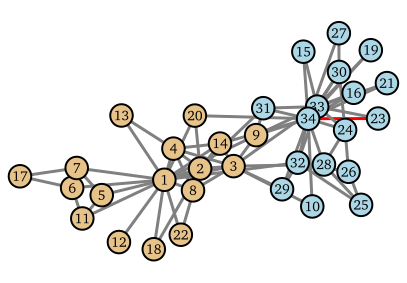
\includegraphics[keepaspectratio]{index_files/mediabag/content/0-intro_files/figure-latex/codefigs-graphs-fig-karate-club-output-1.pdf}}

}

\caption{\label{fig-karate-club}Zachary's Karate Club, with ambiguously
extant edge 78 highlighted.}

\end{figure}%

\emph{We do not know if any of these are true}. In fact, as illustrated
in Figure~\ref{fig-karate-club}, we do not know if the network being
described from the original edge data even has 77 or 78 edges, due to
ambiguous reporting in the original work. Lacking a precise definition
of what the graph's components (i.e.~it's edges) are, \emph{as
measurable entities}, means we cannot estimate the measurement error in
the graph.

\section{Indirect Network
Measurement}\label{indirect-network-measurement}

While the karate club graph has unquantified edge uncertainty derived
from ambiguous edge measurements, we are fortunate that we \emph{have
edge measurements}. Regardless of how the data was collected, it is de
facto reported as a list of pairs. In many cases, we simply do not have
such luxury. Instead, our edges are only measured \emph{indirectly}, and
instead we are left with lists of node co-ocurrences. Networks
connecting movies as being ``similar'' might be derived from data that
lists sets of movies watched by each user; networks of disease spread
pathways might be implied from patient infection records; famously, we
might build a network of collaboration strength between academic authors
by mining datasets of the papers they co-author together.

Such networks are derived from what we will call \emph{node activation}
data, i.e., records of what entities happened ``together'', whether
contemporaneously, or in some other context or artifact.

\begin{figure}

\centering{

\pandocbounded{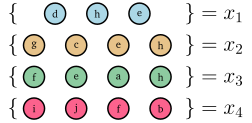
\includegraphics[keepaspectratio]{index_files/mediabag/content/0-intro_files/figure-latex/codefigs-graphs-fig-obs-set-output-1.pdf}}

}

\caption{\label{fig-obs-set}}

\end{figure}%

These are naturally represented as ``bipartite'' networks, having
separate entites for, say, ``papers'' and ``authors'', and connecting
them with edges (paper 1 is ``connected'' to its authors E,H,C, etc.).
But analysts are typically seeking the collaboration network connecting
authors (or papers) themselves! Networks of relationships in this
situation are not directly observed, but which \emph{if recovered} could
provide estimates for community structure, importances of individual
authors (e.g.~as controlling flow of information), and the ``distances''
that separate authors from each other, in their respective domains.
\autocite{Scientificcollaborationnetworks._Newman2001} Common practice
assumes that co-authorship in any paper is sufficient evidence of at
least some level of social ``acquaintance'', where more papers shared
means more ``connected''.

\begin{figure}

\centering{

\pandocbounded{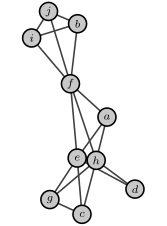
\includegraphics[keepaspectratio]{index_files/mediabag/content/0-intro_files/figure-latex/codefigs-graphs-fig-collab-output-1.pdf}}

}

\caption{\label{fig-collab}}

\end{figure}%

Thus our social collaboration network is borne out of indirect
measurements: author connection is implied through ``occasions when
co-authorship occurred''. However, authors of papers may recall times
that others were added, not by their choice, but by someone else already
involved. In fact, the final author list of most papers is reasonably a
result of individuals choosing to invite others, not a unanimous,
simultaneous decision by all members. Let's imagine we wished to study
the social network of collaboration more directly: if we had the luxury
of being in situ as, say, a sociologist performing an academic
ethnography, we might have been more strict with our definition of
``connection''. If the goal is a meaningful social network reflecting
the strength of interraction between colleages, perhaps the we prefer
our edges represent ``mutual willingness to collaborate''. Edge
``measurement'', then, could involve records of events that show
willingness to seek or participate in collaboration event, such as:

\begin{itemize}
\tightlist
\item
  \emph{author (g) asked (e), (h), and (c) to co-author a paper, all of
  whom agreed}
\item
  \emph{(i) asked (f) and (j), but (j) wanted to add (b)'s expertise
  before writing one of the sections}
\end{itemize}

and so on. Each time two colleagues had an opportunity to work together
\emph{and it was seized upon} we might conclude that evidence of their
relationship strengthed. With data like this, we could be more confident
in claiming our collaboration network can serve as ``ground truth,'' as
far as empirically confirmed collaborations go. However, even if the
underlying ``activations'' are identical, our new, directly measured
graph looks very different.

\begin{figure}

\centering{

\pandocbounded{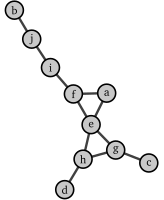
\includegraphics[keepaspectratio]{index_files/mediabag/content/0-intro_files/figure-latex/codefigs-graphs-fig-colleague-output-1.pdf}}

}

\caption{\label{fig-colleague}graph of mutual collaboration
relationships i.e.~the ``ground truth'' social network}

\end{figure}%

Fundamentally, the network in Figure~\ref{fig-colleague} shows which
relationships the authors \emph{depend} on to accomplish their
publishing activity. When causal relations between nodes are being
modeled as edges, we call such a graph a \emph{dependency network}. We
will investigate this idea further later on, but ultimately, if a
network of dependencies is desired (or implied, based on analysis
needs), then the critical problem remaining is \emph{how do we recover
dependency networks from node activations?} Additionally, what goes
wrong when we use co-occurence/activation data to estimate the
dependency network, especially when we wish to use it for metrics like
centrality, shortest path distances, and community belonging?

\begin{figure}

\centering{

\pandocbounded{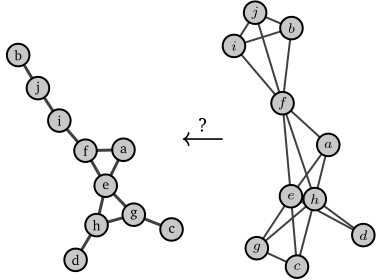
\includegraphics[keepaspectratio]{index_files/mediabag/content/0-intro_files/figure-latex/codefigs-graphs-fig-recover-output-1.pdf}}

}

\caption{\label{fig-recover}Recovering underlying dependency networks
from node-cooccurrences.}

\end{figure}%

Even more practically, networks created directly from bipartite-style
data are notorious for quickly becoming far too dense for useful
analysis, earning them the (not-so-)loving moniker ``hairballs''.
Network ``backboning,'' as it has come to be called tries to find a
subset of edges in this hairball that still captures it's core topology
in a way that's easier to
visualize.\autocite{twostagealgorithm_Slater2009,backbonebipartiteprojections_Neal2014}
Meanwhile, underlying networks of dependencies that \emph{cause} node
activation patterns can provide this: they are almost always more sparse
than their hairballs. Accessing the dependency \emph{backbone} in a
principled way is difficult, but doing so in a rapid, scalable manner is
critical for practitioners to be able to make use of it to trim their
hairballs.

\section{Scope of this work}\label{scope-of-this-work}

The purpose of this thesis is to provide a solid foundation for basic
edge metrology when our data consists of binary node activations, by
framing network analysis as a problem of \emph{inference}, as suggested
by \textcite{Statisticalinferencelinks_Peel2022}. We give special focus
to binary activations that occur due to spreading processes, such as
random walks or cascades on an underlying carrier graph. Recovering the
carrier, or, ``dependency'' network from node activations is of great
interest to the network backboning and causal modeling communities, but
often involves either unspoken sources of epistemic and aleatory error,
or high computation costs (or both). To begin addressing these issues,
we present a guide to current practices, pitfalls, and how common
statistical tools apply to the network recovery problem: a
\emph{Practitioner's Guide to Network Recovery}. We cover what
``measurement'' means in our context, and specifically the ways we
encode observations, operations, and uncertainties numerically.
Clarifying what different versions of what ``relation'' means (whether
proximity or incidence) is critical, since network structure is intended
to encode such relations as mathematical objects, despite common
ambiguities and confusion around what practitioners intend on
communicating through them. Then we use this structure to present a
cohesive framework for selecting a useful network recovery technique,
based on the available data and where in the data processing pipeline is
acceptable to admit either extra modeling assumptions or information
loss.

Next, building on a gap found in the first part, we present a novel
method, \emph{Forest Pursuit}, to extract dependency networks when we
know a \emph{spreading process} causes node activation (e.g.~paper
co-authorship caused by collaboration requests). We create a new
reference dataset to enable community benchmarking of network recovery
techniques, and use it show greatly improved accuracy over many other
widely-used methods. Forest Pursuit in its simplest form scales linearly
with the size of active-node sets, being trivially parallelizable and
streamable over dataset size, and agnostic to network size overall. We
then expand our analysis to re-imagine Forest Pursuit as a Bayesian
probabilistic model, \emph{Latent Forest Allocation}, which has an
easily-implemented Expectation Maximization scheme for posterior
estimation. This significantly improves upon the accuracy results of
Forest Pursuit, at the cost of some speed and scalability, giving
analysts multiple options to adapt to their needs.

Last, we apply Forest Pursuit to several qualitative case-studies,
including a scientific collaboration network, and the verbal fluency
``animals'' network recovery problem, which dramatically change
interpretation under use of our method. We investigate its use as a
low-cost preprocessor for other methods of network recovery,like GLASSO,
improving their stability and interpretability. Finally we discuss the
special case when node activations are reported as an ordered set, where
accounting for cascade-like effects becomes crucial to balance false
positive and false-negative edge prediction. Along with application of
this idea to knowledge-graph creation from technical language in the
form maintenance work-order data, we discuss more broadly the future
needs of network recovery, specifically in the context of embeddings and
gradient-based machine learning toolkits.

\part{A Practitioner's Guide to Network Recovery}

\chapter{Metrology with matrices}\label{metrology-with-matrices}

Where metrology is concerned, the actual unit of observation and how it
is encoded for us is critical to how analysts may proceed with
quantifying, modeling, and measuring uncertainty around observed
phenomena. Experiment and observation tends to be organized as inputs
and outputs, or, independent variables and dependent variables,
specifically. Independent variables are observed, multiple times
(``observations''), and changes in outcome for each can be compared to
the varying values associated with the independent variable input
(``features''). For generality, say a practitioner records their
measurements as scalar values,
i.e.~\(x\in\mathbb{S}\in\{\mathbb{R,Z,N},\cdots\}\). The structure most
often used to record scalar values of \(n\) independent/input variable
features over the course of \(m\) observations is called a design matrix
\(X:\mathbb{S}^{m\times n}\).\footnote{ Not all observations are scalar,
  but they can become so. If individual measurements are
  higher-dimensional (e.g.~images are 2D), X is a tensor, which can be
  transformed through unrolling or embedding into a lower dimensional
  representation before proceeding. There are other techniques for
  dealing with e.g.~categorical data, such as one-hot encoding (where
  the features are binary for each possible category, with boolean
  entries for each observation).}

\section{Observation and feature ``spaces''}\label{sec-matrix-notation}

If we index a set of observations and features, respectively, as
\[ i\in I=\{1,\cdots,m\}, \quad j\in J=\{1,\cdots,n\},\qquad I,J:\mathbb{N}\]
then the design matrix can map the index of an observation and a feature
to the corresponding measurement.
\begin{equation}\phantomsection\label{eq-design-mat}{
x=X(i,j)\qquad X : I\times J \rightarrow \mathbb{S}
}\end{equation} i.e.~the measured value of the \(j\)th independent
variable from the \(i\)th observation.\footnote{ This notation is
  adapted from the sparse linear algebraic treatment of graphs in
  \textcite{GraphAlgorithmsLanguage_Kepner2011} and
  \textcite{MathematicalfoundationsGraphBLAS_Kepner2016}.} In this
scheme, an ``observation'' is a single row vector of features in
\(\mathbb{S}^{n\times 1}\) (or simply \(\mathbb{S}^{n}\)), such that
each observation encodes a position in the space defined by the
features, i.e.~the \emph{feature space}, and extracting a specific
observation vector \(i\) from the entire matrix can be denoted as
\[\mathbf{x}_i=X(i,\cdot),\quad \mathbf{x}:J\rightarrow\mathbb{S}\]
Similarly, every ``feature'' is associated with a single column vector
in \(\mathbb{S}^{1\times m}\), which can likewise be interpreted as a
position in the space of observations (the \emph{data space}):
\[\mathbf{x}_j'=X(\cdot,j),\quad \mathbf{x}':I\rightarrow\mathbb{S}\]
Note that this definition could be swapped without loss of generality.
In other words, \(\mathbf{x}\) and \(\mathbf{x}'\) being in row and
column spaces is somewhat arbitrary, having more to do with the
logistics of experiment design and data collection. We could have
measured our feature vectors one-at-a-time, measuring their values over
an entire ``population'', in effect treating that as the independent
variable set.\footnote{ In fact, vectors are often said to be in the
  column-space of a matrix, especially when using them as
  transformations in physics or deep learning layers. We generally
  follow a one-observation-per-row rule, unless otherwise stated.}

To illustrate this formalism in a relevant domain, let's take another
look at co-citation networks. For \(m\) papers we might be aware of
\(n\) total authors. For a given paper, we are able to see which authors
are involved, and we say those authors ``activated'' for that paper. It
makes sense that our observations are individual papers, while the
features might be the set of possible authors. However, we are not given
information about which author was invited by which other one, or when
each author signed on. In other words, the measured values are strictly
boolean, and we can structure our dataset as a design matrix
\(X:\mathbb{B}^{m\times n}\). We can then think of the
\(i^{\mathrm{th}}\) paper as being represented by a vector
\(\mathbf{x}_i:\mathbb{B}^n\), and proceed using it in our various
statistical models. If we desired to analyze the set of authors, say, in
order to determine their relative neighborhoods or latent author
communities, we could equally use the feature vectors for each paper,
this time represented in a vector
\(\mathbf{x}'_j:\mathbb{B}^{1\times m}\).

\section{Models \& linear operators}\label{sec-lin-ops}

Another powerful tool an analyst has is \emph{modeling} the observation
process. This is relevant when the observed data is hypothesized to be
generated by a process we can represent mathematically, but we do not
know the parameter values to best represent the observations (or the
observations are ``noisy'' and we want to find a ``best'' parameters
that account for this noise). This is applicable to much of scientific
inquiry, though one common use-case is the de-blurring of observed
images (or de-noising of signals), since we might have a model for how
blurring ``operated'' on the original image to give us the blurred one.
We call this ``blurring'' a \emph{linear operator} if it can be
represented as a matrix\footnote{in the finite-dimensional case}, and
applying it to a model with \(l\) parameters is called the \emph{forward
map}:
\[\mathbf{x} = F\mathbf{p}\qquad F:\mathbb{R}^{l}\rightarrow \mathbb{R}^n\]
where \(P\) is the space of possible parameter vectors, i.e.~the
\emph{model space}. The forward map takes a modeled vector and predicts
a location in data space.

Of critical importance, then, is our ability to recover some model
parameters from our observed data, e.g.~if our images were blurred
through convolution with a blurring kernel, then we are interested in
\emph{deconvolution}. If \(F\) is invertible, the most direct solution
might be to apply the operator to the data, as the \emph{adjoint map}:
\[ \mathbf{p} = F^H\mathbf{x}\qquad F^H:\mathbb{R}^{n}\rightarrow \mathbb{R}^l\]
which removes the effect of \(F\) from the data \(\mathbf{x}\) to
recover the desired model \(\mathbf{p}\).

Trivially we might have an orthogonal matrix \(F\), so \(F^H=F^{-1}\) is
available directly. In practice, other approaches are used to minimize
the \emph{residual}:
\(\hat{\mathbf{p}}^=\min_{\mathbf{p}} F\mathbf{p}-\mathbf{x}\). Setting
the gradient to 0 yields the normal equation, such that
\[ \hat{\mathbf{p}}=(F^TF)^{-1}F^T\mathbf{x}\] This should be familiar
to readers as equivalent to solving ordinary least-squares (OLS).
However, in that case it is more often shown as having the \emph{design
matrix} \(X\) in place of the operator \(F\).

\emph{This is a critical distinction to make:} OLS as a ``supervised''
learning method treats some of the observed data we represented as a
design matrix previously as a target to be modeled, \(y=X(\cdot,j)\),
and the rest maps parameters into data space, \(F=X(\cdot,J/j)\). With
this paradigm, only the target is being ``modeled'' and the rest of the
data is used to create the operator. In the citation network example, it
would be equivalent to trying to predict one variable, like citation
count or a specific author's participation in every paper, \emph{given}
every other author's participation in them.

For simplicity, most work in the supervised setting treats the reduced
data matrix as X, opting to treat \(y\) as a separate \emph{dependent
variable}. However, our setting will remain \emph{unsupervised}, since
no single target variable is of specific interest---all observations are
``data''. In this, we more closely align with the deconvolution
literature, such that we are seeking a model and an operation on it that
will produce the observed behavior in an ``optimal'' way.

\section{Measurement quantification \& error}\label{sec-smooth-err}

In binary data, such as what we have been considering, it is common to
model observables as so-called ``Bernoulli trials'': events with two
possible outcomes (on, off; yes, no; true, false), and one outcome has
probability \(p\). These can be thought of as weighted coin-flips:
``heads'' with probability \(p\), and ``tails'' \(1-p\). If \(k\) trials
are performed (the ``exposure''), we say the number of successes \(s\)
(the ``count'') is distributed as a binomial distribution
\(s\sim Bin(p,k)\). The empirical estimate for the success probability
is \(\hat{p}=\tfrac{s}{k}\).

Note that this naturally resembles marginal sums on our design matrix
\(X\), if we treat columns (or rows!) as an array of samples from
independent Bernoulli trials:
\(\hat{p}_j = \frac{\sum_{i\in I} X(i,j)}{m}\). Many probability
estimates involving repeated measurements of binary variables (not
simply the row/column variables) have this sort of
\(\frac{\textrm{count}}{\textrm{exposure}}\) structure, as will become
useful in later sections.

However, if we are ``measuring'' a probability, we run into issues when
we need to quantify our uncertainty about it. For instance, an event
might be quite rare, but if in our specific sample we \emph{never} see
it, we still do not generally accept a probability of zero.

\subsection{Additive Smoothing}\label{sec-counting}

One approach to dealing with this involves adding \emph{pseudocounts}
that smooth out our estimates for count/exposure, from which we get the
name ``additive smoothing''.{[}CITE?{]}
\[\hat{p} = \frac{s+\alpha}{k+2\alpha} \] Adding 1 success and 1 failure
(\(\alpha=1\)) as pseudocounts to our observations is called
\emph{Laplace's Rule of Succession}, or simply ``Laplace
smoothing,''\footnote{ derived when Laplace desired estimates of
  probability for unobserved phenomena, such as the sun (not) rising
  tomorrow.} while adding \(\alpha=0.5\) successes and failures is
called using \emph{Jeffrey's Prior}. It's so-called because this
pseudocount turns out to be a special case of selecting a Beta prior on
the Bernoulli probability \(p\sim \textrm{Beta}(\alpha, \beta)\), such
that the posterior distribution for \(p\) after our observations is
\(\textrm{Beta}(s+\alpha, k-s+\beta)\), which has the mean:
\begin{equation}\phantomsection\label{eq-beta-binomial}{
E[p|s,k]=\frac{s+\alpha}{k-\alpha+\beta}
}\end{equation}

This exactly recovers additive smoothing with a Jeffrey's prior for
\(\alpha=\beta=0.5\).\footnote{ A useful comparison of the two priors
  (1, 0.5) is to ask, given all of the trials we have seen so far,
  whether we believe we are near the ``end'' or ``middle'' of an average
  run of trials. For \(\alpha=1\), we believe nearly all evidence has
  been collected, but for \(\alpha=0.5\), only half of expected evidence
  has been observed.\\
} This generalization allows us to be more flexible, and specify our
prior expectations on counts or exposure with more precision. Such
models provide both an estimate of the aleatory uncertainty (via the
posterior distribution), and a form of ``shrinkage'' that prevents
sampling noise from unduly affecting parameter estimates (via the prior
distribution). Despite being a simple foundation, this treatment of
``counts'' and ``exposure'' can be built upon in many ways.

\subsection{Conditional Probabilities \&
Contingencies}\label{conditional-probabilities-contingencies}

In dependency/structure recovery, since our goal involves estimating (at
least) pairwise relationships, the independence assumption required to
estimate node occurrences as Beta-Binomial is clearly
violated.\footnote{ In fact, a recent method from
  \autocite{MultivariateBernoullidistribution_Dai2013} models
  probabilistic binary observations, \emph{with dependencies}, by
  generalizing the mechanics overviewed here to a fully multivariate
  Bernoulli distribution, capable of including 3rd- and higher-order
  interractions, not just pairwise.\\
}

However, it's common to estimate how similar two random variables
\(A,B\) are, e.g.~if samples of each correspond to columns of binary
\(X\). For instance, the joint probabilities \(P(A\cap B)\) answer ``how
often does A happen with B, out of all data?'' Conditional probabilities
\(P(A|B)=\frac{P(A\cap B)}{P(B)}\) measure how often A occures given B
happened. Once again, we can estimate the base probabilities \(P(A)\)
and \(P(B)\) with methods like Equation~\ref{eq-beta-binomial} for each
marginal sums \(X(\cdot,A)\) or \(X(\cdot,B)\), but the joint and
conditional probabilities can instead be estimated using matrix
multiplication using the Gram matrix, discussed below. It encodes
pair-wise co-occurrence counts, such that
\(G(i,i'):\mathbb{Z}^{n\times n}\) has the co-occurrence count for node
\(i\) with \(i'\).

For binary data, we typically create association meatures from values on
a \(2\times2\) contingency table, with counts and marginals. A shorthand
notation for these values is:

\begin{equation}\phantomsection\label{eq-contingency}{
\begin{array}{c|cc|c}
      & B=1         & B=0         & \sum_B \\
\hline 
A=1   & p_{11}      & p_{10}      & p_{1\bullet} \\
A=0   & p_{01}      & p_{00}      & p_{0\bullet} \\
\hline 
\sum_A   & p_{\bullet 1} & p_{\bullet 0} & p_\bullet \\
\end{array}
}\end{equation}

The co-occurrence probability \(p_{11}=P(A\cap B)\) for each pair can
also be approximated with the beta-binomial scheme mentioned above, but
care must be taken not to confuse this with the edge strength connecting
two nodes. First, nodes that rarely activate (low node probability) may
nonetheless reliably connect to others when they do occur (high edge
probability). In fact, without direct observation of edges, we are not
able to estimate their count, \emph{or} their exposure, which can be a
source of systemic error from \emph{epistemic uncertainty}. We don't
know when edges are used, directly, and we also don't have a reliable
way to estimate the opportunities each edge had to activate (their
exposure), either. This is especially true when we wish to know whether
an edge even \emph{can} be traversed, i.e.~the edge \emph{support}.
Support, as used in this sense, is the set of inputs for which we expect
a non-zero output. Intuitively, this idea captures the sense that we
might care more about \emph{whether} an edge/dependency exists, not
\emph{how important} it is. For that, we have to re-assess our simple
model: even if we could count the number of times an edge might have
been traversed, how do we estimate the opportunities it had to be
available for traversal (it's ``exposure'')?

Assuming this kind of epistemic uncertainty can be adequately addressed
through modeling---attempts at which will be discussed in more detail in
Chapter~\ref{sec-lit-review}---conditional probability/contingency
tables will again be useful for validation. When comparing estimated
edge probability to some known ``true'' edge existence (if we have
that), we can count the number of correct predictions, as well as type I
(false positive) and type II (false negative) errors. We can do this at
\emph{every probability/weight threshold value}, as well, and we will
return to ways to aggregate all of these values into useful scoring
metrics in Section~\ref{sec-FP-experiments}.

\section{Distance vs.~Incidence}\label{sec-products}

As we have already seen, operations from linear algebra make many
counting and combinatoric tasks easier, while unifying disparate
concepts to a common set of mechanics. In addition to having a map from
integer indices to sets of interest, these design matrices/vectors are
implicitly assumed to have entries that exist in a field
\(F=(\mathbb{S},\oplus,\otimes)\). equipped with operators analogous to
addition (\(\oplus\)) and multiplication (\(\otimes\)).\footnote{ Or,
  more generally, a semiring if inverse operations for
  \(\oplus,\otimes\) don't exist.} With this, we are able to define
generalized inner products that take pairs vectors in a vector space
\(\mathbf{x}\in V\), such that
\(\langle\cdot,\cdot\rangle_F:\mathbb{S}^n\times \mathbb{S}^n\rightarrow \mathbb{S}\).
\[
\langle\mathbf{x}_a,\mathbf{x}_b\rangle_{F} = \bigoplus_{j=1}^n \mathbf{x}_a(j)\otimes\mathbf{x}_b(j)
\]

We can use this to perform ``contractions'' along any matching
dimensions of matrices as well, since the sum index is well-defined. \[
\begin{aligned}
X\in\mathbb{S}^{m\times n}\quad Y\in\mathbb{S}^{n\times m} \\
Z(i,j)=X\oplus,\otimes Y = \bigoplus_{j=1}^{n} X(i,j) \otimes Y(j,k) = XY
\end{aligned}
\] For ease-of-use, we will assume the standard field for any given set
\((\mathbb{S},+,\times)\) if not specified otherwise, which recovers
standard inner products \(\langle\cdot,\cdot\rangle\). However,
\textcite{MathematicalfoundationsGraphBLAS_Kepner2016} illustrates the
usefulness of various fields (or semirings). They allow linear-algebraic
representation of many graph operations, such as shortest paths through
inner products over \((\mathbb{R}\cup -\infty,\textrm{min}, +)\). This
works because discrete/boolean edge weights will not accumulate extra
strength beyond 1 under contraction over observations.

\subsection{Kernels \& distances}\label{kernels-distances}

As alluded to in the previous section, co-occurrence have a deep
connection to a Gram matrix, which is a matrix of all pairwise inner
products over a set of vectors.

\begin{equation}\phantomsection\label{eq-gram-mat}{
X^TX=G(j,j')=\langle\mathbf{x'}_j,\mathbf{x}_{j'}'\rangle = \sum_{i=1}^{m} X(i,j)X(i,j')
}\end{equation}

Matrices that can be decomposed into another matrix and its transpose
are symmetric, and positive semidefinite (PSD), making every gram matrix
PSD. They are directly related to (squared) euclidean distances through
the polarization identity{[}CITE?{]}:\footnote{\textbf{Important}: these
  definitions are all using the \(\mathbf{x}'\) notation to indicate
  that these measurements are almost exclusively being done in the
  \emph{data space}, i.e.~on column vectors. While most definitions work
  on distances in terms of the measurements/objects/data, for
  \emph{inverse problems} (like network recovery, structure learning,
  etc.) they are more often applied in terms of the features (here, the
  nodes. This can be seen in statistics as well, where covariance and
  correlation matrices (which are related to the gram and distance
  matrix definitions above), are defined as relationships between
  features/dimensions, not individual samples.}
\begin{equation}\phantomsection\label{eq-sq-distance}{
d^2(j,j') = \|\mathbf{x}_{j'}'-\mathbf{x}_{j'}'\|^2 = G(j,j) - 2G(j,j') + G(j',j') 
}\end{equation}

In our example from before, the gram matrix will have entries showing
the number of papers shared by two authors (or total papers by each, on
the diagonal). This is because an inner product between two author
(column) vectors will add 1 for each paper in the sum only if it has
both authors in common. This is called a \emph{bipartite
projection}{[}CITE{]} into the authors ``mode'', and is illustrated
visually in Figure~\ref{fig-collab}.

Due to {[}CITE Shoenberg/Mercer{]}, we can generalize
Equation~\ref{eq-sq-distance} such that \emph{any} function ``kernel''
function \(\kappa(x,y)\) that creates PSD matrix
\(K(j,j')\in\mathbb{S}^{n\times n}\). It says that such a PSD matrix can
always be decomposed into a form \(K=R^TR\) for any matrix
\(R(i,j)\in \mathbb{S}^{m\times n}\), thus letting us use the
polarization identity to create arbitrary distance metrics. on
\(\mathbb{S}^n\)
\autocite{SimilaritiesgraphsKernels_Avrachenkov2019}\footnote{ Distance
  metric, here, means that \(d(x,y)\) satisfies the triangle inequality
  for all \(x,y\).}
\begin{equation}\phantomsection\label{eq-dist-kernel}{
d_K(j,j') = \tfrac{1}{2}\left(K(j,j)+K(j',j'))\right)-K(j,j')
}\end{equation}

This ability to create valid distance measures from arbitrary kernel
functions is the core of a vast area of machine learning and statistics
that employs the so-called \emph{kernel trick}. {[}CITE?{]} Different
kernels yield different properties useful for distinguishing points
having specific properties. One class of kernels are normalized to the
range \([0,1]\), such that we ensure that equality along any one
dimension is given a weight of \(\tilde{K}(j,j)=1\). Such a kernel
matrix can be derived from any other kernel, and is often combined with
a logarithmic similarity measure \(\tilde{\kappa}(x,y)=\log{s(x,y)}\).
\begin{equation}\phantomsection\label{eq-norm-diag}{
\begin{aligned}
\tilde{K}(j,j') &= \frac{K(j,j')}{\sqrt{K(j,j)^2K(j',j')^2}}\\
d_{\tilde{K}}(j,j') &= -\log{\tilde{K}(j,j')}
\end{aligned}
}\end{equation} Since this is equivalent to applying
Equation~\ref{eq-dist-kernel} to \(s\) directly. This normalization
should be familiar as the way cosine similarities and correlation
matrices are made as well (also having 1s along their diagonal), and
illustrates how non-metric similarities can be potentially made into
(pseudo)metrics.

\subsection{Incidence structures \&
dependency}\label{incidence-structures-dependency}

Rather than how ``close'' or ``far'' to points are in vector space,
which is described with the kernels and distances above, whether
something ``touches''---or, is incident to---something else is usually
described abstractly as an \emph{incidence structure}. This is an
abstract way to describe how things ``touch'', such as when a set of
points lie on a line/plane, or nodes touch an edge. We say an incidence
structure is a triple of sets called (for historical reasons)
\emph{points} \(\mathfrak{P}\), \emph{lines} \(\mathfrak{L}\), and
\emph{flags} \(\mathfrak{I}\).\autocite{Incidencegeometry_Moorhouse2007}
\[(\mathfrak{P,L,I})\quad \mathfrak{I}\subseteq \mathfrak{P}\times\mathfrak{L}\]

Representing these as matrices will be further explored in
Section~\ref{sec-incidence-vec}. But, the discrete nature of these
incidence sets makes it clear that estimating the size and elements of
\(\mathfrak{I}\), is a very different question from estimating the
similarity/distance between two entities in a vector space.

In statistics, such discrete structures usually arise when we are
concerned with direct dependence from indirect. Take as an example a set
of masses connected together by springs. If we shake one mass, all
masses will also shake some amount, depending on the spring constants of
the springs each mass is ``transmitted'' force through, and the losses
due to friction or air resistance. While the amount of movement over
time depends on how ``close'' in this spring network two masses are, the
movement itself can only be transmitted through springs that the masses
are \emph{incident} to. Movement could be modeled through
similarity/distance measurements like correlation, since none of the
masses are independent (all move when any do), but incidence in terms of
spring force transmission is modeled in terms of conditional
(in)dependence. If we hold all but two masses still, and moving one
doesn't move the other, then we know they are conditionally independent:
no spring connects them!

This idea gets formalized as probabilistic graphical models, which are
networks that define ``incidence'' between two variables as conditional
dependence. Letting the random variables in the column-space of \(X\) be
\(A,B\) and the remaining columns be \(C=X(\cdot,J\setminus \{A,B\})\),
then \begin{equation}\phantomsection\label{eq-cond-indep}{
P(A\cap B |C ) = P(A|C)P(B|C)\implies (A\perp B|C)\implies (A,B)\notin \mathfrak{I}
}\end{equation} for a set of incidences \(\mathfrak{I}\) defining a PGM
that was sampled as \(X\).

{[}SPRING GRAPHIC?{]}

\subsection{Conclusion}\label{conclusion}

\chapter{Incidence through vector
representation}\label{incidence-through-vector-representation}

To provide a sufficiently rigorous foundation for network recovery from
binary occurrence, we will need a rigorous way to represent networks and
occurrences that lends itself to building structured ways both connect
to each other. We build on the incidence structure and matrix product
formalism from the previous chapter, introducing various ways to build
graphs as incidence structures that have direct representations as
matrices. This can be extended to representing occurrences as matrices
of \emph{hyperedge vectors}. This view allows us to interpret different
representations of graphs (or hypergraphs) as connected by simple matrix
operations.

Traditionally\autocite{MathematicalfoundationsGraphBLAS_Kepner2016,WhyHowWhen_Torres2021},
we might say a graph on nodes (or, ``vertices'')
\(v\in V=\{1,\cdots,n\}\) and ``edges'' \(E\) is a tuple: \[
G=(V,E) \quad \textrm{s.t.} \quad E\subseteq V \times V
\]

In incidence geometry terms, this would be similar to making two
duplicate sets of the same nodes, and defining a graph as the set of
incidences between nodes. The \emph{adjacency matrix} \(A\) of \(G\),
degree matrix \(D\), and graph/discrete Laplacian \(L\) are then defined
as:\footnote{ The \emph{indicator function} \(\mathbf{1}_A(x)\) is 1 for
  values of \(x\) in the set \(A\), and 0 otherwise.} \[
\begin{aligned}
A(u,v) & =\mathbf{1}_E((u,v)) \quad &A : V\times V\rightarrow \mathbb{B} \\
D(u,v) & =\mathrm{diag}({\textstyle\sum}_V A(u,v))\quad &D : V\times V\rightarrow \mathbb{N} \\
L(u,v) & = D(u,v) - A(u,v) \quad &L : V\times V\rightarrow \mathbb{Z} 
\end{aligned}
\]

However, if edges and their recovery is so important to us, defining
them explicitly as nodes-node incidences can be problematic when we wish
to estimate edge existence (or not), given noisy pairs of node
co-occurrences. Additionally, we have to be very careful to distinguish
whether our graph is \emph{(un)directed}, \emph{weighted},
\emph{simple}, etc., and hope that the edge set has been filtered to a
subset of \(N\times N\) for each case. Instead, we propose a less
ambiguous framework for vectorizing graphs, based on their underlying
incidence structure.

\section{Graphs as incidence structures}\label{sec-incidence-vec}

Instead, we give edges their own set of identifiers,
\(e\in E=\{1,\cdots \omega\}\). Now, define graphs as incidence
structures between nodes and edges such that every edge is incident to
either two nodes, or none:

\begin{equation}\phantomsection\label{eq-simple-incidence}{
G = (V,E,\mathcal{I}) \quad s.t. \quad \mathcal{I} \subseteq E\times V
}\end{equation}

Variations on graphs can often be conveniently defined as constraints on
\(\mathcal{I}\):

\begin{itemize}
\tightlist
\item
  Self loops can be prohibited by only allowing unique flags for a given
  relation\footnote{ never two flags with the same pair,
    i.e.~\(\mathcal{I}\) is a set, not a multiset.}
\item
  Multigraphs are similarly described by whether we allow pairs of
  vertices to appear with more than one edge\footnote{ in the set of
    flags containing nodes \(u\) or \(v\), only one \(e\) may be
    incident to both of them.}
\end{itemize}

Together, these constraints define ``simple'' graphs. Similarly, we can
equip Equation~\ref{eq-simple-incidence} with a function \(B\) that
allows \(\mathcal{I}\) to encode information about the specific kinds of
incidence relations under discussion. We give \(B\) a range of possible
flag values \(S\):

\begin{equation}\phantomsection\label{eq-map-incidence}{
G = (V,E,\mathcal{I},B) \quad s.t. \quad \mathcal{I} \subseteq E\times V\quad B:\mathcal{I}\rightarrow S
}\end{equation}

\begin{itemize}
\tightlist
\item
  Undirected, unweighted graphs only need single elements: ``incidence
  exists'' i.e.\(S=\{1\}\)
\item
  Directed graphs can use two elements e.g.~a ``spin'' for
  \(S=\{-1,1\}\)
\item
  Weighted, undirected graphs are supported on positive scalars
  e.g.~\(S=\mathbb{R}^+\)
\item
  Weighted, directed graphs are supported on any scalar
  e.g.~\(S=\mathbb{R}_{\neq0}\)
\end{itemize}

If the ``absence'' of incidence needs to be modeled explicitly, a
``null'' stand-in (0,False) can be added to each \(S\), which is useful
for representing each structure as arrays for use with linear algebra
(i.e.~\(\{0,1\}\),\(\{-1,0,-1\}\),\(\mathbb{R}^+_0\), and
\(\mathbb{R}\), respectively). By doing so, we can also place an exact
limit on the maximum possible size of \(\omega=\|E\|\) in the simple
graph case, and indicate edges by their unique ID, such that
\(\mathcal{I}= E\times V\) is no longer a subset relation for
\(E=\{1,\cdots,{n\choose2} \}\). Instead of existence in
\(\mathcal{I}\), we explicitly use incidence relation \(S\) to tell us
whether each possible edge ``exists'' or not, simplifying our graph
definition further\footnote{ if we allomulti-edges , then}:

\begin{equation}\phantomsection\label{eq-incidence-graph}{
\begin{gathered}
G  = (V,E,B) \quad s.t. \quad B : E\times V \rightarrow S\\
v \in V = \{1,\cdots, n\}\quad \\
e \in E = \left\{1,\cdots, {n\choose 2} \right\}
\end{gathered}
}\end{equation}

The representation of \(B\) in Equation~\ref{eq-incidence-graph} bears a
remarkable similarity to our original description of design matrices in
Equation~\ref{eq-design-mat}. In fact, as a matrix, \(B(e,v)\) is called
the \emph{incidence} matrix: every row has two non-zero entries, with
every column containing a number of non-zero entries equal to that
corresponding node's degree in \(G\). Traditionally, we use an
\emph{oriented} incidence matrix, such that each row has exactly one
positive (non-zero) value, and one negative (non-zero) value.\footnote{
  In fact, this would make B\^{}*(v,e) equivalent to a \emph{graphical
  matroid}, another common formalism that generalizes graph-like
  structures to vector space representations.} Even for undirected
graphs, the selection of \emph{which entry} is positive or negative is
left to be ambiguous, since much of the math used later is symmetric
w.r.t. direction\footnote{though not always!}.

\subsection{Embedding incidences in vector
space}\label{embedding-incidences-in-vector-space}

A formalism for graphs that starts with incidence matrices would benefit
from a \emph{canonical} oriented incidence matrix, rather than the
family that is ambiguous w.r.t. edge orientation. To start, we can be
more precise by selecting each row(edge) vector, and partitioning it
into two: one for each non-zero column (node) that edge is incident to.
Every incidence can be represented individually as standard basis vector
\(\mathbf{e}\) in the feature space of \(B\), scaled by the
corresponding value of \(S\).

Let \(V_e\) be the set of nodes with (non-zero) incidence to edge \(e\).
Then the incidence vectors are:\\
\begin{equation}\phantomsection\label{eq-incidence-vec}{
\delta_e(v) = B(e,v)\mathbf{e}_v \quad \forall v\in V_e
}\end{equation} And the (unoriented) incidence matrix vectors are
recovered as sums over the incidence vectors for each edge:
\begin{equation}\phantomsection\label{eq-incidence-edge-sum}{
\mathbf{b}_e = \sum_{v\in V_e} \delta_e(v)
}\end{equation}

A traditional approach might then define undirected graphs as
equivalent, in some sense, to multidigraphs, where each edge is really
two directed edges, in opposing directions. This does allow the matrix
\(B\) to have the correct range for its entries in this formalism (the
directed graph range, \(S=\{-1,0,1\}\)), and the edge identity based on
sums would hold. However, the resulting set of incidences would have
twice the number of edges than our combinatoric limit for simple graphs,
and prevent the more elegant definition of graph types through the set
\(\mathbf{S}\). Plus, it would necessitate averaging of weights over
different edge ID's to arrive at a single undirected ``edge weight'',
and many other implementation details that make keeping track of
specifics difficult for practitioners.

Instead, we would like a canonical oriented distance matrix, which can
be derived from the vectorized incidences in the undirected range of
\(B\) (the standard basis vectors). Without loss of generality, let
\(u_e,v_e\in V_e\) be nodes such that \(u<v\).\footnote{the inequality
  is strict because self-loops are not allowed.} Using this, we can
unambiguously define a \emph{partition}
\(B(e,\cdot)=B(e,u_e) + B(e,v_e)\) between incidences on \(e\), along
with a new derived incidence, \(B_o\), which has oriented rows like:
\[B_o(e,\cdot)=\mathbf{b}^o_e = \delta_e(u)-\delta_e(v)\] In other
words, while the unoriented incidence matrix is the ``foundational''
representation for graphs in our formalism, the (canonical) oriented one
can be derived, even if negative incidence values are not in
\(\mathbb{S}\).\footnote{ This works as long as we are in at least a
  ring, since semirings in general do not need to define additive
  inverse operations. In this case we would limit ourselves to the
  oriented incidence.}

But, now that we have removed the information on ``which nodes an edge
connects'' from our definition of edges (since every edge is a scalar
ID), how do we construct \(V_e\) without a circular dependency on \(B\)
to find non-zero entries? Because of our unique identification of edges
up to the combinatoric limit, we can still actually provide a unique
ordering of the nodes in \(V_e\), without searching over the entirety of
\(B\)'s domain. Using an identity from
\textcite{ParallelEuclideandistance_Angeletti2019}, we have a
closed-form equation both to retrieve the IDs of nodes \(u,v\) (given an
edge \(e\)), and an edge \(e\) (given two nodes \(u,v\)), for any simple
graph with \(n\) vertices.
\begin{equation}\phantomsection\label{eq-sq-id}{
\begin{gathered}
    u_n(e) = n - 2 - \left\lfloor\frac{\sqrt{-8e + 4n(n - 1) - 7}-1}{2}\right\rfloor\\
    v_n(e) = e + u_n(e) + 1 -\frac{1}{2} \left(n (n - 1) + (n - u_n(e))^2 - n+u_n(e)\right)\\
    e_n(u,v) = \frac{1}{2}\left(n(n - 1) - ((n - u)^2 - n+u)\right) + v - u - 1
\end{gathered}
}\end{equation} Our ease-of-calculation lets us drop some of the excess
notation and refer to our (un)oriented incidence matrices in terms of
the incidences of each edge on their \(u\) or \(v\), directly. \[
B = B_u + B_e \qquad B_o \equiv B_u - B_v
\]

\subsection{\texorpdfstring{Inner products on
\(B\)}{Inner products on B}}\label{inner-products-on-b}

With all of this background, the other representations of graphs can
seen as derivations from the canonical incidence matrices. The
Laplacian, which is usually introduced either in terms of
ajacency/degree, or as the gram matrix for oriented edge vectors, is
also related to the gram matrix between all pairs of incidences on
\((u,v)\). The other identities are simply consequences of the
polarization identity:
\begin{equation}\phantomsection\label{eq-laplacian}{
\begin{split}
L & = B_o^TB_o\\
  & = \|B_u - B_v \|^2 \\
  & = 2\|B_u\|^2 +2\|B_v\|^2 - \|B_u + B_v \|^2 \\
  & = 2D - B^TB = D-A
\end{split}
}\end{equation}

The Laplacian is often used in defining random-walks and markov chains,
such that the degree of each node should be normalized to 1, which can
be accomplished either by row- or column-normalizing it:
\(L^{\textrm{rw}}=D^{-1}L\) or \(LD^{-1}\), respectively. If this
degree-normalization is desired without de-symmetrizing \(L\), we can
still perform an operation similar to normed kernels in
Equation~\ref{eq-norm-diag}, called the symmetric normalized Laplacian.
\begin{equation}\phantomsection\label{eq-norm-laplacian}{
\tilde{L} = D^{-\tfrac{1}{2}}LD^{-\tfrac{1}{2}} = \frac{L(u,v)}{\sqrt{L(u,u)^2L(v,v)^2}}
}\end{equation}

\subsection{Edge Metrology, Edge
Vectors}\label{edge-metrology-edge-vectors}

Implicitly in the use of \(B\) with design matrix mechanics from the
previous chapter is a treatment of edges as ``observations'' (the data
space), and nodes as features. If an edge \emph{is} an observation, then
unfortunately we cannot really quantify uncertainty over repeated
measurements of edges with the simple mechanics from
Section~\ref{sec-counting} (because that edge \emph{is} that
corresponding observation, and IDs are not duplicated).

So far we have seen two ways of representing the entire graph in matrix
form: Incidence matrix \(B\) (or \(B_o\)), and the inner-product
matrices derived from it (\(L\), \(A\)). Since we can recover node IDs
from edge IDs by Equation~\ref{eq-sq-id}, we can use a single vector to
represent an entire graph structure by it's edges alone. Then a data
dimension for vectors in ``edge space'' can once again represent
observations, with nodes implied by Equation~\ref{eq-sq-id}. This is
either done by contracting \(B\) along the nodes (columns) dimension, or
by \emph{unrolling} the upper triangle of \(L\) or \(A\) according to
Equation~\ref{eq-sq-id}.\footnote{ Equation~\ref{eq-edge-vectors} uses
  an averaging operation to accomplish the contraction, but any
  reduction over the two nodes shared by an edge would accomplish the
  same, especially since we rarely see separate values for edge weight
  per-node, the way incidences can.} If each vector represents a value
of \(B\) associated with a corresponding edge, then \(m\) of these
vectors would be equivalent to \(m\) observations of \({n \choose 2}\)
edges on the same set of \(n\) nodes. Formally, for the \(i\)th observed
structure on \(n\) nodes:
\begin{equation}\phantomsection\label{eq-edge-vectors}{
\begin{gathered}
R(i,e) = \min(\{B_i(e, u_n(e)),B_i(e,v_n(e))\}) \\
\quad \textrm{s.t.} \quad R:I\times E \rightarrow \mathbb{S}\\
i\in I = \{1,\cdots,m\} \qquad e \in E=\left\{1,\cdots,\omega\right\}\\
n=\tfrac{1}{2}(1+\sqrt{8\omega+1})
\end{gathered}
}\end{equation} This representation formalizes what practitioners call
``edgelists'' into a data structure that can unambiguously distinguish
directed, undirected, and weighted graphs. In addition, it allows for
repeated measurements of edges over the same set of nodes, while
flexibly growing when new nodes arrive.\footnote{ For instance, say
  observations are stored as sparse entries via \(R\), and a new node
  arrives. First, the participating nodes can be recovered in a
  vectorized manner through Equation~\ref{eq-sq-id}. Then, a new node id
  increases \(n\), followed by reassignment of the edge IDs with
  \(e_n(u,v)\).}

\section{Generalized node occurrence
vectors}\label{generalized-node-occurrence-vectors}

TODO

\begin{figure}[H]

{\centering \pandocbounded{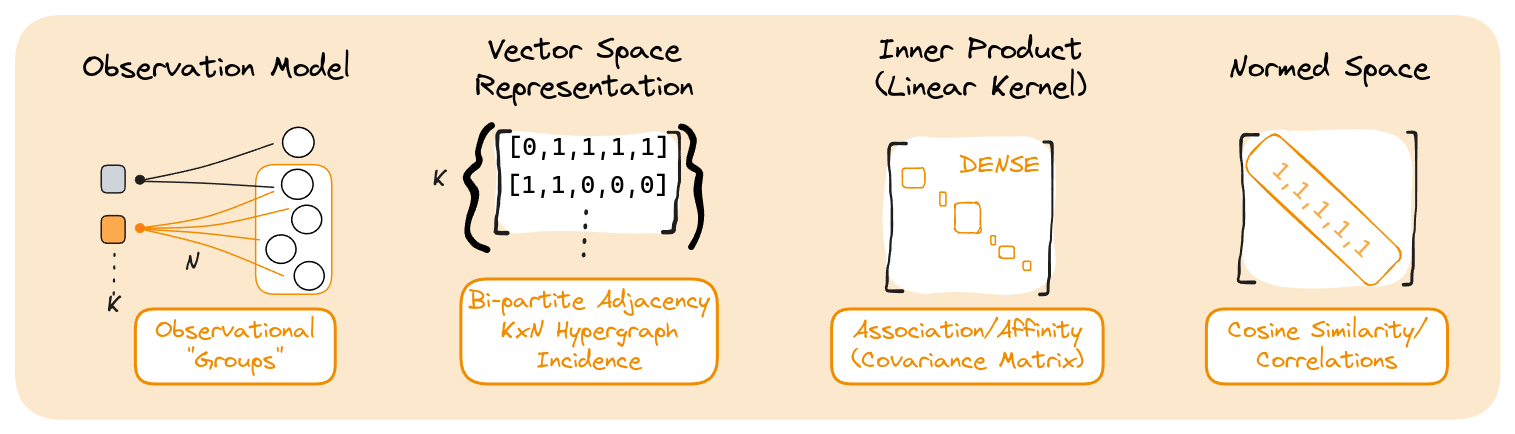
\includegraphics[keepaspectratio]{content/part1/../images/hypergraph-observations.png}}

}

\caption{Hyperedge Relation Observational Model}

\end{figure}%

\subsection{Hyperedges as vectors of node
occurrence}\label{hyperedges-as-vectors-of-node-occurrence}

\begin{figure}

\begin{minipage}{0.50\linewidth}

\centering{

\[
%X(\{1,2,3,4,\cdots\})=\\
\begin{array}{c c}
& \begin{array}{cccccccccc} a & b & c & d & e & f & g & h & i & j\\ \end{array} \\
\begin{array}{c c } x_1\\x_2\\x_3\\x_4\\ \vdots \end{array} &
\left[
\begin{array}{c c c c c c c c c c}
  0  &  0  &  1  &  0  &  1  &  0  &  1  &  1  &  0  &  0 \\
  1  &  0  &  0  &  0  &  1  &  1  &  0  &  0  &  0  &  0 \\
  0  &  1  &  0  &  0  &  0  &  1  &  0  &  0  &  1  &  1 \\
  0  &  0  &  0  &  1  &  1  &  0  &  0  &  1  &  0  &  0 \\
  &&&& \vdots &&&&&
\end{array}
\right]
\end{array}
\]

}

\subcaption{\label{fig-biadj-mat}}

\end{minipage}%
%
\begin{minipage}{0.50\linewidth}

\centering{

\pandocbounded{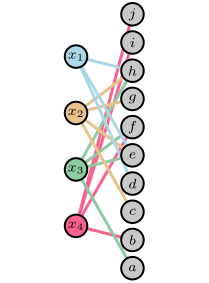
\includegraphics[keepaspectratio]{index_files/mediabag/content/part1/1-02-graph-obs_files/figure-latex/..-codefigs-graphs-fig-bipartite-output-1.pdf}}

}

\subcaption{\label{fig-bipartite}Bipartite representation of node
``activation'' data}

\end{minipage}%

\end{figure}%

\subsection{Inner product on
Hyperedges}\label{inner-product-on-hyperedges}

Roundabout way of describing binary/occurrence data. Inner product is
co-occurrences.

Leads to correlation/covariance, etc.

\subsection{Combining Occurrence \&
Dependence}\label{combining-occurrence-dependence}

\begin{itemize}
\tightlist
\item
  soft cosine
\item
  kernels on graphs (incl.~coscia euclidean)
\item
  Linear operator incidences
\item
  Retrieving one from the other is hard.
\end{itemize}

\chapter{Roads to Network Recovery}\label{sec-lit-review}

Here we give a brief overview of the key approaches to backboning and
dependency reovery for networks through binary activations. This is by
far an incomplete overview, though other existing approaches are likely
to fall within the provided outline due to its generality. Finally, we
assess patterns in the assumptions made by the presented algorithms, and
motivate a new one to fill a gap perceived in the network recovery
space.

\section{Organizing Recovery Methods}\label{organizing-recovery-methods}

All recovery methods will require assumptions in addition to data to
accomplish their task. As discussed in \textcite{WhyHowWhen_Torres2021},
there are fundamental difference in dependency capability between the
network and hypergraphic/bipartite representations of complex systems.
Necessarily, some information will be lost in translation between the
two forms.

As a (hopefully) helpful way to organize the various \emph{kinds} of
assumptions that are taking bipartite observations to simple graphs, we
present an organization of common modeling assupmtions into three
loosely-defined groups:

\begin{itemize}
\tightlist
\item
  Local Structure \& Additivity
\item
  Information Flow \& Resource Constraints
\item
  Global Structure Models
\end{itemize}

In truth, this classification should be viewed as more of a sliding
scale, with approaches falling somewhere within. Some approaches make
very few assumptions about the shape a resulting network ``should''
take, but do so by making strong assumptions about how individual
observations relate to a desired quantity, and especially how those
observations are able to be combined to result in an ``answer'', however
that looks. Others instead provide clear normative constraints on the
overall network topology, or emission mechanism, but this allows for
flexibility in how data is individually handled.

This idea could be thought of as similar to pooling in bayesian
inference. Do individuals all have fundamentally separate distributions,
so that global behavior (and by extension, uncertainty) is an aggregate
phenomena? Or do individuals inherit parameters from a global
distribution shared by all, and anything outside that structural
assumption must be ``noise''? In between the extremes, some other
assumption as to how the global and local scales mitigate information
between them is required, i.e.~\emph{partial pooling}. In this domain,
what we often see are attempts to perform noise corrections through the
way information is thought to travel between nodes, generally.

For each, we provide examples to illustrate modeling patterns and
highlight common practice, though for a deeper assessment of the broad
space of backboning and edge prediction in general a reader may see the
overview in \textcite{atlasaspiringnetwork_Coscia2021}.

\subsection{Local Structure \& Additivity
Assumptions}\label{local-structure-additivity-assumptions}

These are, together, typically called ``association'' measures. While
they are sometimes presented as functions of the entire dataset, they
nearly always find a basis in the inner-product operation, and have
definitions in terms of \emph{contractions} along the data/observation
dimension. By relying on the (Euclidean) inner product, even with
various re-weighting or normalization schemes, an analyst is making
strong assumptions about their ability to reliably take measurements
from linear combinations of observed activation vectors.

Essentially, if a measure relies on marginal counts or summation over
the data axis, then the main assumptions are at the \emph{local} level,
about whether what we are adding together estimates our target
correctly. The most basic would be to count co-occurrences, and
consequently the co-occurrence probability \(p_{11}=P(A,B)\). However,
for very rare co-occurrences, we need to correct for rate-imbalance of
the nodes in much the same way correlation normalizes covariance. This
idea leads to ``cosine similarity''

\begin{tcolorbox}[enhanced jigsaw, opacityback=0, colback=white, left=2mm, arc=.35mm, colframe=quarto-callout-note-color-frame, breakable, toprule=.15mm, rightrule=.15mm, bottomrule=.15mm, leftrule=.75mm]

\quartocallouttip{tip-cs} 

\vspace{-3mm}\textbf{Tip \ref*{tip-cs}: Ochiai Coefficient
(Cosine){[}@Measuresecologicalassociation\_Janson1981{]}}\vspace{3mm}

Effectively an uncentered correlation, but for binary observations the
``cosine similarity'' is also called the \emph{Ochiai Coefficient}
between two sets \(A,B\), where binary ``1'' stands for an element
belonging to the set. In our use case, it is measured as \[
\frac{|A \cap B |}{\sqrt{|A||B|}}=\sqrt{p_{1\bullet}p_{\bullet 1}} \rightarrow  \frac{X^TX}{\sqrt{\mathbf{s}_i\mathbf{s}_i^T}}\quad \mathbf{s}_i = \sum_i \mathbf{x}_i
\]

\end{tcolorbox}

This interpretation of cosine similarity as the geometric mean of
conditional probabilities is particularly useful when trying to
approximate interaction rates. The geometric mean as a pooling operator
is conserved through Bayesian updates
\autocite{ProbabilityAggregationMethods_Allard2012}, so the use of a
prior with co-occurrences as base counts is possible for additive
smoothing. To do this, the goemetric mean of marginal counts acts as a
``psedovariable'' for exposure somewhere between A and B. Empirically,
this is a powerful approximation with good performance characteristics,
for relatively little effort.

\begin{tcolorbox}[enhanced jigsaw, opacityback=0, colback=white, left=2mm, arc=.35mm, colframe=quarto-callout-note-color-frame, breakable, toprule=.15mm, rightrule=.15mm, bottomrule=.15mm, leftrule=.75mm]

\quartocallouttip{tip-or} 

\vspace{-3mm}\textbf{Tip \ref*{tip-or}: Odds Ratios}\vspace{3mm}

Along with others derived from it, the Odds ratio is based on the ratio
of conditional probabilities, and takes the form
\[\text{OR}=\frac{p_{11}p_{00}}{p_{01}p_{10}}\] Yule's Q and Y
\autocite{MethodsMeasuringAssociation_Yule1912} are mobius transforms of
the (inverse) \(\text{OR}\) and \(\sqrt{\text{OR}}\), respectively, that
map association values to \([-1,1]\).
\[Q = \frac{\text{OR}-1}{\text{OR}+1}\quad Y=\frac{\sqrt{\text{OR}}-1}{\sqrt{\text{OR}}+1}\]

\end{tcolorbox}

Odds ratio is important to logistic regression, where the coefficients
are usually the log-odds ratios of occurrence vs.~not
(\(\log{\text{OR}}\)).\\
Yule's Y, also called the ``coefficient of colligation'', tends to scale
with association strength in an intuitive way, so that proximity to 1 or
-1 paints a more useful picture than the odds-ratio alone.

Another association measure, based in information theory, asks ``how
much can I learn about one variable by observing another?''

\begin{tcolorbox}[enhanced jigsaw, opacityback=0, colback=white, left=2mm, arc=.35mm, colframe=quarto-callout-note-color-frame, breakable, toprule=.15mm, rightrule=.15mm, bottomrule=.15mm, leftrule=.75mm]

\quartocallouttip{tip-mi} 

\vspace{-3mm}\textbf{Tip \ref*{tip-mi}: Mutual information}\vspace{3mm}

An estimate for the mutual information (i.e.~between the sample
distributions) can be derived from the marginals, as above, though it is
more compactly represented as a pairwise sum over the domains of each
distribution being compared: \[
\text{MI}(A,B)\approx \sum_{i,j\in[0,1]} p_{ij} \log \left( \frac{p_{ij}}{p_{i\bullet}p_{\bullet j}} \right) 
\]

\end{tcolorbox}

It is non-negative, with 0 occurring when A and B are independent. There
are many other information-theoretic measures related to MI, but we
specifically bring this up as it will be the basis for the Chow Liu
method, later on.

Sometimes, especially in social networks, we might want to avoid
overcounting relationships with very well-connected nodes. This was
brought up with respect to the normalized Laplacian before, but we could
also perform a normalization on the underlying bipartite adjacencies.

\begin{tcolorbox}[enhanced jigsaw, opacityback=0, colback=white, left=2mm, arc=.35mm, colframe=quarto-callout-note-color-frame, breakable, toprule=.15mm, rightrule=.15mm, bottomrule=.15mm, leftrule=.75mm]

\quartocallouttip{tip-hyp} 

\vspace{-3mm}\textbf{Tip \ref*{tip-hyp}: Hyperbolic Projection}\vspace{3mm}

Attempts to account for the overcounting of co-occurrences on frequently
occurring nodes, vs.~rarer
ones.\autocite{Scientificcollaborationnetworks._Newman2001}
\[ X^T\text{diag}(1+\mathbf{s}_j)^{-1}X \quad \mathbf{s}_j = \sum_j{\mathbf{x}_j'}\]
This reweights each observation by its degree in the original biartite
graph.

\end{tcolorbox}

So far this is the first measure that re-weights observations
\emph{before} contraction, so that it depends on having the individual
observations available (rather than only the gram matrix). In this case,
each observation's entries are all equally re-weighted by the number of
activations in it (each nodes ``activation fraction'' in that
observation).

\subsection{Resource and Information
Flow}\label{resource-and-information-flow}

These methods are somewhere between local and global constraint scales.
This is accomplished by imagining nodes as having some amount of a
resource (like information or energy) and correcting for observed noise
in edge activation by reinforcing the \emph{geodesics} that most likely
transmitted that resource.

First, closely related to hyperbolic re-weighting, we can imagine the
bipartite connections as evenly dividing each nodes' resources, before
reallocating them to the nodes they touch, in turn. For instance, we
might say each author splits their time among all of the papers they are
on, and in turn every co-author ``receives'' an evenly divided
proportion of everyone's time they are co-authoring with.

\begin{tcolorbox}[enhanced jigsaw, opacityback=0, colback=white, left=2mm, arc=.35mm, colframe=quarto-callout-note-color-frame, breakable, toprule=.15mm, rightrule=.15mm, bottomrule=.15mm, leftrule=.75mm]

\quartocallouttip{tip-rp} 

\vspace{-3mm}\textbf{Tip \ref*{tip-rp}: Resource Allocation}\vspace{3mm}

Goes one step further than hyperbolic projection, by viewing each node
as having some ``amount'' of a resource to spend, which gets
re-allocated by observational unit.
\autocite{Bipartitenetworkprojection_Zhou2007}
\[ \text{diag}(\mathbf{s}_i)^{-1}X^T\text{diag}(\mathbf{s}_j)^{-1}X \]

\end{tcolorbox}

Interestingly, we could see this as a two-step random-walk normalization
of the bipartite adjacency matrix \[
\begin{pmatrix}
0_{n,n} & X^T \\
X & 0_{m,m}
\end{pmatrix}
\] First the row-normalized, then the column-normalized. This matrix is
asymmetric, so a symmetric edge strength estimate is often retrieved by
mean, max, or min reduction operations.

Rather than stop after two iterations, continuing to enforce unit
marginals to convergence is known as the Sinkhorn-Knopp algorithm, which
converges to a doubly-stochastic matrix (both marginal directions sum to
1).

\begin{tcolorbox}[enhanced jigsaw, opacityback=0, colback=white, left=2mm, arc=.35mm, colframe=quarto-callout-note-color-frame, breakable, toprule=.15mm, rightrule=.15mm, bottomrule=.15mm, leftrule=.75mm]

\quartocallouttip{tip-ot} 

\vspace{-3mm}\textbf{Tip \ref*{tip-ot}: Doubly Stochastic}\vspace{3mm}

If \(A\in \mathbb{S}^{n\times n}\) is positive, then there exists
\(d_1,d_2\) such that \[W=\text{diag}(d_1)A\text{diag}(d_2)\] is
doubly-stochastic, and \(W(u,v)\) is the \emph{optimal transport plan}
between \(u\) and \(v\) with regularized Euclidean distance between them
on a
graph.\autocite{RobustInferenceManifold_Landa2023,Sinkhorndistanceslightspeed_Cuturi2013}

The doubly-stochastic filter removes edges from \(W\) until just before
the graph would become disconnected.

\end{tcolorbox}

As the name implies, the optimal transport plan reflects the minimum
cost to move some amount of resource from one node to another. By
focusing on best-case cost, we enforce a kind of ``principle of least
action'' to bias recovery toward edges along these geodesics.

A more direct way to do this, perhaps, is to find the shortest paths
from every node to each other node, and aggregate them.

\begin{tcolorbox}[enhanced jigsaw, opacityback=0, colback=white, left=2mm, arc=.35mm, colframe=quarto-callout-note-color-frame, breakable, toprule=.15mm, rightrule=.15mm, bottomrule=.15mm, leftrule=.75mm]

\quartocallouttip{tip-hss} 

\vspace{-3mm}\textbf{Tip \ref*{tip-hss}: High-Salience Skeleton}\vspace{3mm}

Count the number of shortest-path trees an edge participates in, out of
all the shortest-path-tres (one for every node).
\[ \frac{1}{n}\sum_{i=1}^n \mathcal{T}_{\text{sp}}(i) \] where
\(\mathcal{T}_{\text{sp}}(n)\) is the shortest-path tree rooted at \(n\)
\autocite{Robustclassificationsalient_Grady2012}Intuition that the most
important edges are on geodesics for many paths blah

\end{tcolorbox}

Unfortunately, HSS is forced to scale with the number of nodes, and must
calculate the entire spanning tree for each one.

\subsection{Global Structural
Assumptions}\label{global-structural-assumptions}

Often times these constraints are as simple as ``the underlying
dependency graph must belong to a family \(\mathcal{C}\)'' of graphs.
Observations are thought of as emissions from a set of node
distributions, where edges are representations of dependency
relationship between them. To provide a foundation to formalize this
notion, one framework is that of Markov Random Fields, which are
undirected generalizations of bayes nets {[}CITE?{]} that use edges to
encode \emph{conditional dependence} between node distributions.

One of the original structures for MRFs that we could recover from
observed data was a \emph{tree}.

\begin{tcolorbox}[enhanced jigsaw, opacityback=0, colback=white, left=2mm, arc=.35mm, colframe=quarto-callout-note-color-frame, breakable, toprule=.15mm, rightrule=.15mm, bottomrule=.15mm, leftrule=.75mm]

\quartocallouttip{tip-chowliu} 

\vspace{-3mm}\textbf{Tip \ref*{tip-chowliu}: Chow-Liu Spanning Tree}\vspace{3mm}

Enforces tree structure globally. Approximates a joint probability \[
P\left(\bigcap_{i=1}^n v_i\right) \approx P' = \prod_{e\in T} P(u_n(e)|v_n(e)) \quad T\in \mathcal{T}
\] where \(\mathcal{T}\) is the set of spanning trees for the nodes. The
Chow-Liu tree minimizes the Kullback-Leibler (KL) Divergence
\(\text{KL}(P \| P')\) by finding the minimum spanning tree over
pairwise mutual information
weights.\autocite{Approximatingdiscreteprobability_Chow1968}

\end{tcolorbox}

Recent work has made it possible to enforce spanning tree structure
while efficiently performing monte-carlo-style bayesian inference, which
estimates a distribution over spanning trees that explain observed
behavior, and by extension the likelihood each edge is in one of these
trees. \autocite{BayesianSpanningTree_Duan2021}

\begin{tcolorbox}[enhanced jigsaw, opacityback=0, colback=white, left=2mm, arc=.35mm, colframe=quarto-callout-note-color-frame, breakable, toprule=.15mm, rightrule=.15mm, bottomrule=.15mm, leftrule=.75mm]

\quartocallouttip{tip-glasso} 

\vspace{-3mm}\textbf{Tip \ref*{tip-glasso}: Covariance Shrinkage \& GLASSO}\vspace{3mm}

in Binary case
\autocite{Sparseinversecovariance_Friedman2008,Structureestimationdiscrete_Loh2012}

Semidefinite program to find (regularized) max. likelihood precision of
Normal Distribution:

\[\operatorname*{argmax} \mathcal{L}(\Theta|\hat{\Sigma})
  = \operatorname*{argmin}_{\Theta \prec 0}\ \text{tr}(\hat{\Sigma} \Theta) - \log |\Theta|+ \rho\|\Theta\|_1 \]

\begin{itemize}
\item
  minimize \(\|\cdot\|_F\) (sample) covariance
  \(\hat{\Sigma}\in \mathbb{R}^{N\times N}\) and a proposed precision
  \(\Theta\)
\item
  higher (log)-determiniant is better
\item
  penalize 1-norm (i.e.~the Lasso)

  also, stability selection
\end{itemize}

\end{tcolorbox}

\begin{tcolorbox}[enhanced jigsaw, opacityback=0, colback=white, left=2mm, arc=.35mm, colframe=quarto-callout-note-color-frame, breakable, toprule=.15mm, rightrule=.15mm, bottomrule=.15mm, leftrule=.75mm]

\quartocallouttip{tip-degseq} 

\vspace{-3mm}\textbf{Tip \ref*{tip-degseq}: Degree Sequence Ensembles}\vspace{3mm}

\autocite{backbonebipartiteprojections_Neal2014,Comparingalternativesfixed_Neal2021}

\end{tcolorbox}

\begin{tcolorbox}[enhanced jigsaw, opacityback=0, colback=white, left=2mm, arc=.35mm, colframe=quarto-callout-note-color-frame, breakable, toprule=.15mm, rightrule=.15mm, bottomrule=.15mm, leftrule=.75mm]

\quartocallouttip{tip-sbm} 

\vspace{-3mm}\textbf{Tip \ref*{tip-sbm}: (Inverse) Stochastic Block Model}\vspace{3mm}

\autocite{ReconstructingNetworksUnknown_Peixoto2018,NetworkReconstructionCommunity_Peixoto2019}

\end{tcolorbox}

\section{A Path Forward}\label{a-path-forward}

\subsection{Tracing Information Loss
Paths}\label{tracing-information-loss-paths}

Table of Existing Approaches

\begin{table}

\caption{\label{tbl-roads}Organizing recovery methods by representation
space and level}

\centering{

\subcaption{\label{tbl-roads-1}}

\centering{

\pandocbounded{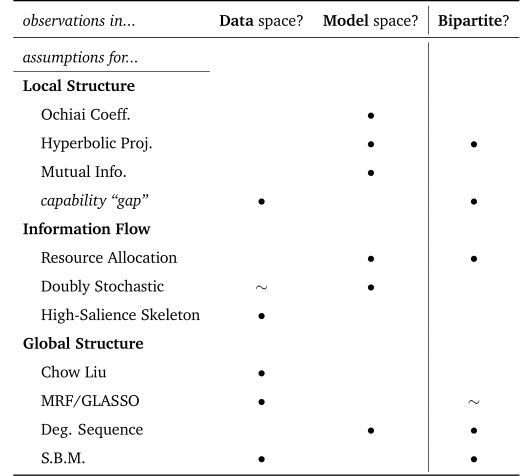
\includegraphics[keepaspectratio]{index_files/mediabag/content/part1/1-03-recovery-road_files/figure-latex/..-codefigs-graphs-tbl-roads-output-1.pdf}}

}

}

\end{table}%

\begin{itemize}
\tightlist
\item
  Observation-level loss (starting with the inner product or kernel)
\item
  Non-generative model loss (no projection of data into model space)
\item
  no uncertainty quantification
\end{itemize}

\subsection{Something New}\label{something-new}

Sorting algorithms\ldots{} \emph{none address all three!}

i.e.~MOTIVATES FOREST PURSUIT

\part{Nonparametric Network Recovery With Random Spanning Forests}

\chapter{Graph Reduce \& Desire Paths}\label{graph-reduce-desire-paths}

Addressing gaps discussed in the previous section to reach a generative
model for network recovery requires careful attention to the generation
mechanism for node activations. While there are many ways we might
imagine bipartite data to be be generated, presuming the existence of a
dependency graph that \emph{causes} activation patterns will give us
useful ways to narrow down the generative specification.

First, we will investigate the common assumption that pairwise
co-occurrences can serve as proxies for measuring relatedness, and how
this ``gambit of the group'' is, in fact, a strong bias toward dense,
clique-filled recovered networks. Because we wish to model our node
activations as being \emph{caused} by other nodes (that they depend on),
we draw a connection to a class of models for \emph{spreading}, or,
\emph{diffusive processes}. We outline how random-walks are related to
these diffusive models of graph traversal, enabled by an investigation
of the graph's ``regularized laplacian'' from
\textcite{Semisupervisedlearning_Avrachenkov2017}. Then we use the
implicit causal dependency tree structure of each observation, together
with the Matrix Forest Theorem
\autocite{MatrixForestTheorem_Chebotarev2006,Countingrootedforests_Knill2013}
to more generally define our generative node activation model. This
leads to a generative model for binary activation data as rooted random
spanning forests on the underlying dependency graph.

\section{The Gambit of the Inner
Product}\label{the-gambit-of-the-inner-product}

As we saw repeatedly in Chapter~\ref{sec-lit-review}, networks are
regularly assumed to arise from co-occurrences, whether directly as
counts or weighted in some way. This assumption can be a significant a
source of bias in the measurement of edges. \emph{Why} a flat count of
co-occurrence leads to ``hairballs'' and bias for dense clusters can be
related to the use of inner products on node activation vectors.

\subsection{Gambit of the Group}\label{gambit-of-the-group}

It seems reasonable, when interactions are unobserved, to assume some
evidence for all possible interactions is implied by co-occurrence.
However, similar to the use of uniform priors in other types of
inference, if we don't have a good reason to employ a fully-connected
co-occurrence prior on interaction dependencies, we are adding
systematic bias to our inference. Whether co-occurrence observations can
be used to infer interaction networks directly was discussed at length
in \textcite{Techniquesanalyzingvertebrate_Whitehead1999}, where
Whitehead and Dufault call this the \emph{gambit of the group}.

\begin{quote}
So, consiously or unconsciously, many ethnologists studying social
organization makr what might be called the ``gambit of the group'': the
assume that animals which are clustered {[}\ldots{]} are interacting
with one another and then use membership of the same cluster
{[}\ldots{]} to define association.
\end{quote}

This work was rediscovered in the context of measuring assortativity for
social networks,\footnote{Assortativity is, roughly, the correlation
  between node degree and the degrees of its neighbors.} where the
author of \textcite{PerceivedAssortativitySocial_Fisher2017} advises
that ``group-based methods'' can introduce sampling bias to the
calculation of assortativity, namely, systematic overestimation when the
sample count is low.

The general problems with failing to specify a model of what ``edges''
actually \emph{are} get analyzed in more depth in
\textcite{Statisticalinferencelinks_Peel2022}. They include a warning
not to naively use correlational measures with a threshold, since even
simple 3-node systems will easily yield false positives edges. Still, it
would be helpful for practitioners to have a more explicit mental model
of \emph{why} co-occurence-based models yield systematic bias,

\subsection{Inner-Product Projections and ``Clique
Bias''}\label{inner-product-projections-and-clique-bias}

Underlying correlation and co-occurrence models for edge strength is a
reliance on inner products between node occurrence vectors. They all use
gram matrices (or centered/scaled versions of them), which were brought
up in Section~\ref{sec-products}. The matrix multiplication performed
represents inner products between all pairs of feature vectors. For
\(X(i,j)\in\mathbb{B}\), these inner products sum together the times in
each observation that two nodes were activated together.

\begin{figure}

\centering{

\pandocbounded{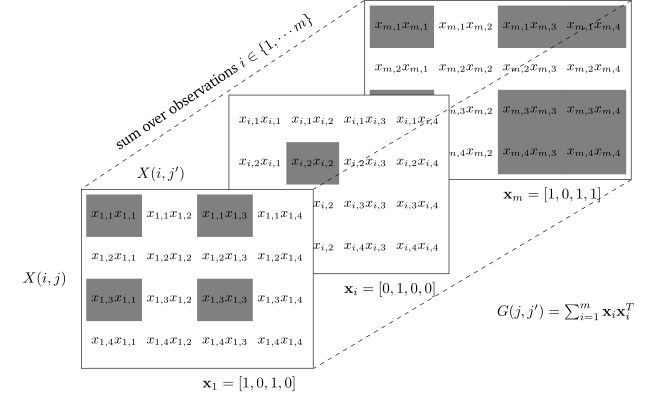
\includegraphics[keepaspectratio]{index_files/mediabag/content/part2/2-01-rand-sf_files/figure-latex/..-codefigs-graphs-fig-stack-outerprod-output-1.pdf}}

}

\caption{\label{fig-stack-outerprod}Gram matrix as sum of observation
outer products}

\end{figure}%

However, another (equivalent) way to view matrix multiplication is as a
sum of outer products \[
G(j,j') = X^T X = \sum_{i=1}^m X(i,j)X(i,j')= \sum_{i=1}^m \mathbf{x}_i\mathbf{x}_i^T
\] Those outer products of binary vectors create \(m\times m\) matrices
that have a 1 in every \(i,j\) entry where nodes \(i,j\) both occurred,
shown in Figure~\ref{fig-stack-outerprod}. Each outer product is
effectively operating as a \(D_i+A_i\) with degrees normalized to 1. If
the off-diagonals can be seen as adjacency matrices, they would strictly
represent a clique on nodes activated in the \(i\)th observation In this
sense, any method that involves transforming or re-weighting a gram
matrix, is implicitly believing that the \(k\)th observation was a
\emph{complete graph}. This is illustrated in
Figure~\ref{fig-stacked-graphs}.

\begin{figure}

\begin{minipage}{0.33\linewidth}

\centering{

\pandocbounded{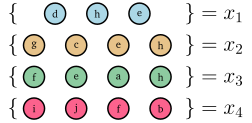
\includegraphics[keepaspectratio]{index_files/mediabag/content/part2/2-01-rand-sf_files/figure-latex/..-codefigs-graphs-fig-obs-set-output-1.pdf}}

}

\subcaption{\label{fig-obs-set}}

\end{minipage}%
%
\begin{minipage}{0.67\linewidth}

\centering{

\pandocbounded{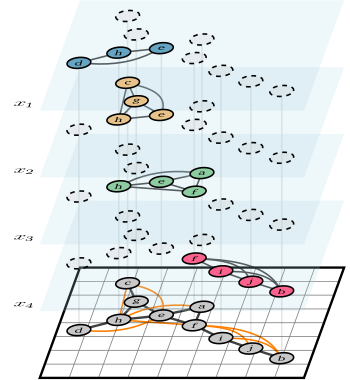
\includegraphics[keepaspectratio]{index_files/mediabag/content/part2/2-01-rand-sf_files/figure-latex/..-codefigs-graphs-fig-stack-bow-output-1.pdf}}

}

\subcaption{\label{fig-stack-bow}Edge Measurements with Group Gambit
(BoW) assumption}

\end{minipage}%

\caption{\label{fig-stacked-graphs}Inner-product projections as sums of
cliques illustrating ``clique bias''.}

\end{figure}%

For many modeling scenarios, this paradigm allows practitioners to make
a more straight-forward intuition-check: do clique observations
\emph{make sense} here? When a list of authors for a paper is finished,
does that imply that all authors mutually interacted with all others
directly to equally arrive at the decision to publish? This would be
similar to assuming the authors might simultaneously enter the same
room, look at a number of others (who all look exclusively at each
other, as well), and \emph{all at once} decide to publish together. In
our introduction, we described a more likely scenario we could expect
from an observer on the ground: a researcher asks a colleague or two to
collaborate, who might know a couple more with relevant expertise, and
so on.

\section{Networks as Desire Path Density
Estimates}\label{networks-as-desire-path-density-estimates}

Unfortunately, methods based on inner-product thresholding are still
incredibly common, in no small part due to how \emph{easy} it is to
create them from occurrence data, regardless of this ``clique-bias''.
The ability to map an operation onto every observation, e.g.~in
parallel, and then reduce all the observations into an aggregate edge
estimate is a highly desirable algorithmic trait. This may be a reason
so many projection and backboning techniques attempt two re-weight (but
retain) the same basic structure, time and again.

What we need is a way to maintain the ease-of-use of inner-product
network creation:

\begin{itemize}
\tightlist
\item
  map an operation onto each observation
\item
  reduce to an aggregate edge guess over all observations
\end{itemize}

but with a more domain-appropriate operator at the observation level.

Let's start with replacements for the clique assumption. There are many
non-clique classes of graphs we might believe local interactions occur
on: path-graphs, trees, or any number of graphs that reflect the topolgy
or mechanism of local interactions in our domain of interest. Authors
have proposed classes of graphs that mirror human perception of set
shapes {[}RELATIVE NEIGHBORHOOD{]}\footnote{ e.g.~for dependencies based
  on perception, such as human decision making tendencies, or causes
  based on color names.}, or graphs whose modeled dependencies are
strictly planar {[}planar maximally filtered graps{]}\footnote{
  e.g.~when interactions are limited to planar dependencies, like
  inferring ancient geographic borders.}. Alternatively, the
interactions might be scale free, small-world, trees, or samples from
stochastic block models.{[}CITE{]} In any case, these assumptions
provide an explicit way to describe the set of \emph{possible}
interaction graphs we believe our individual observations are sampled
from.

\subsection{Subgraph Distributions}\label{sec-subgraph-dists}

Let's use the notation from Equation~\ref{eq-edge-vectors}, such that
each observation of nodes \(\mathbf{x}_i\) is implicitly derived from a
set of activated edges \(\mathbf{r_i}\). To start, our current belief
about what overall structure the whole network can take is
\(G^*=(V,E,B^*)\), where \(B^*\) might always return \(1\) to start out
(the complete graph). To further constrain the problem, let us assume
that node activation is noiseless: any activated nodes were truly
activated, and unactivated nodes were truly inactive (no false negative
or false positive activations).\footnote{ Hidden nodes (unobserved nodes
  beyond the \(n\)) are outside the scope of this work, though could
  potentially be implied for certain structures e.g.~when the metric is
  known to be tree-like. \textcite{TreeIam_Sonthalia2020} use a greedy
  embedding that minimizes distortion to estimate the need for added
  \emph{Steiner} nodes.} So, each \(\mathbf{x}_i\) will induce a
subgraph \(g_i = G^*[V_i]\), where
\(V_i = \{v\in \mathcal{V} | X(i,\mathcal{V})=1\}\). Then, our domain
knowledge takes the form of a constraint on edges within that subgraph,
which will induce a family of subgraphs on \(g_i\). This family
\(\mathcal{C}_i\) belongs to the relevant class of graphs
\(\mathcal{C}\), limited to nodes \(V_i\), i.e.

\begin{equation}\phantomsection\label{eq-subgraph-family}{
\begin{gathered}
\mathcal{C}_i = \{(V,E,B_i) \in\mathcal{C}|B_i(e,v)=B^*(e,v)\mathbf{1}_{V_i}(v)\mathbf{1}_{E_i}(e)\}\\
E_i\in\{\mathcal{E}\in\mathcal{P}(E)| g_i[\mathcal{E}]\in\mathcal{C}\}
V_i = \{v\in \mathcal{V} | X(i,\mathcal{V})=1\}
\end{gathered}
}\end{equation}\footnote{\(\mathcal{P}(A)\) is the \emph{powerset} of
  \(A\), i.e.~the set of all subsets of \(A\).}

In other words, the edges that ``caused'' to the node activations in a
given observation must \emph{together} belong to a graph that, in turn,
belongs to our desired class, which must occur on the nodes that were
activated.

Assuming we can define an associated measure \(\mu_i(c)\) onfor each
\(c\in\mathcal{C}_i\), we are able to define a probability distribution
over subgraphs in the class.\footnote{ This is certainly not a trivial
  assumption, and might either be ill-defined or require techniques like
  the Gumbel trick\autocite{GradientEstimationStochastic_Paulus2020} to
  approximate, unless the partition function \(\mathbb{Z}\) has a closed
  form, or \(\mu\) is already a probability measure on some
  \(\sigma\)-algebra over \(\mathcal{C}\). Closed-form \(\mathcal{Z}\)
  values on \(\mathcal{C}\) are known for a handful of graph classes,
  such as the space of spanning trees, \(\mathcal{C}=\mathcal{T}\).
  However, another way this might be accomplished is through random
  geometric graphs{[}CITE{]}, or geometric spanners like
  Urqhart{[}CITE{]} and Relative Neighborhood {[}CITE{]} graphs on a
  ``sprinkling'' of points that preserves their observed pairwise
  distances.\\
  This is further discussed in Section~\ref{sec-future-hyperbolic}.}
Using notation similar to distributions over spanning trees in
\textcite{EfficientComputationExpectations_Zmigrod2021}:

\begin{equation}\phantomsection\label{eq-subgraph-prob}{
\begin{gathered}
p_i(c) = \frac{\mu_i(c)}{\mathbb{Z}_i}\\
\mathbb{Z}_i = \sum_{c\in\mathcal{C}_i} \mu_i(c)
\end{gathered}
}\end{equation}

This can be represented using the vectorization in
Equation~\ref{eq-edge-vectors}, due to the one-to-one correspondence
established, so that, with a slight abuse of notation treating
\(\mathcal{C}_i\) as the parameter of distribution \(p_i\):
\begin{equation}\phantomsection\label{eq-edgevec-prob}{
\mathbf{r}_{i}(e)|\mathbf{x_i} \sim p_i(\mathcal{C},E,V)
}\end{equation}

So we may not have an exact vector, but we have established a way to
specify a family of edge vectors that could be responsible. With
\(p_i(c)\), we also have a mechanism to sample them when a partition
function is available (or able to be approximated).

With these mechanics in place, we see the choice of a clique (implied by
the inner product) is a trivial application of
Equation~\ref{eq-edgevec-prob}, since that is equivalent to selecting
the class of cliques on \(V_i\) nodes. This has only one element
(\(\|\mathcal{C}_{\text{clique}}\|=1\)), there is only 1 possible
selection, with probability \(p_i(K^{V_i})=1\).

\subsection{Graph Unions as Desire
Paths}\label{graph-unions-as-desire-paths}

With a distribution over subgraphs each observation, we are potentially
able to sambple from them for bootstrap or Monte Carlo estimation
purposes, or simply find a maximum likelihood estimate for each
distribution. Assuming this is true, we may now sample or approximate a
matrix \(R(i,e):I\times E \rightarrow \mathbb{B}\).\\
Methods for doing this efficiently in certain cases are the focus of
Section~\ref{sec-FP} and Section~\ref{sec-lfa-gibbs}. However, once
\(R(i,e)\) is estimated, a reasonable mechanism for estimating the
support of the set of edges is to use
\(\frac{\text{count}}{\text{exposure}}\), but with a few needed
modifications.

First, while the nodes counts in \(\sum_i B(i,\cdot)\) are by assumption
\emph{not} independent, or even pairwise independent, the \emph{edge
traversal} counts \(\sum_i R(i,\cdot)\) could more reasonably be
considered so. A model certainly could be constructed where edge
existence depends on other edges existing (or not). But nothing is
inherently self-inconsistent with a model that assumes the
traversability of individual edges will be independent of one another.

let P(e) be the probability that an edge is traversed (in any
observation), and P(u,v) the probability that nodes \(u,v\) co-occur. To
approximate the overall traversability of an edge, we can calculate an
empirical estimate for the conditional probability
\(P(e|(u,v))=\frac{P(e)\cap P(u,v)}{P(u,v)}\) that an edge is traversed,
given that the two incident nodes are activated. This estimate can use
the same beta-bernoulli distribution from
Equation~\ref{eq-beta-binomial}.

Still, how do we ensure our estimate is approximating traversability, so
that the probability that an edge probability converges toward 1 as long
as it \emph{has to be possible} for \(e\) to be traversed? Recall from
the introduction that, from a measurement perspective, the underlying
networks rarely ``exist'' in the sense that we never truly find the
underlying network, but only samples from (or caused by) it. Imagine
that the ``real'' network is a set of paved sidewalks: our procedure is
similar to watching people walk along paths between locations, and
wanting to estimate which of the paths would be tread ``enough'' to be
paved. This is where we build on an intuition based on the popular idea
of \emph{desire paths} which is a colloquial name for paths that form
when individuals walk over grass or dirt enough to carve a trail. In
network analysis and recovery, we usually are only allowed to see the
desire paths that might have formed from our data, never the actual
``pavement''.

If presented with two equivalent paths, an individual is likely to
choose the one that has been tread more often before i.e.~the ``more
beaten'' path. So, we don't want a probability that an edge has been
traversed, but a probability over fractions of the time we expect an
edge to have been traversed \emph{more often than not}: how likely it is
to ``be beaten''. This is accomplished by forcing \(\alpha, \beta < 1\).
For the case where \(\alpha=\beta=0.5\), we call this special case an
\emph{arcsine} distribution.

In a coin tossing game where each ``heads'' gives a point to player A
and ``tails'' to player B, then the point differential is modeled as a
random walk. The arcsine distribution
\(\text{Beta}(\tfrac{1}{2},\tfrac{1}{2})\) is exactly the probability
distribution for the fraction of time we expect one player to be
``ahead'' of the other. \autocite{WhatisArcsine_Ackelsberg2018}

\begin{quote}
``\emph{Contrary to popular opinion, it is quite likely that in a long
coin-tossing game one of the players remains practically the whole time
on the winning side, the other on the losing side.''}

William Feller\autocite[Chapter
III]{IntroductionProbabilityTheory_Feller1968}
\end{quote}

This is desirable behavior for a distribution over edge traversability!
We expect the vast majority of edges to have a 0 or 1 as the most likely
values, with the expected fraction of observations that an edge being
traversed was ``ahead'' of it being \emph{not} traversed matching our
empirical count. We generalize this with \(\alpha = 1-\beta\), with
\(\alpha + \beta = 1\), such that the new beta posterior from
Equation~\ref{eq-beta-binomial} with \(s\) successes over \(k\) trials
is:

\begin{equation}\phantomsection\label{eq-desirepath-binom}{
\begin{gathered}
\pi \sim \text{Beta}(\alpha + c, 1-\alpha-c) \\
c = \frac{s-ak}{k+1}\\
\end{gathered}
}\end{equation}

Important to note is that \(k\) is measured over the
\emph{co-occurrences} \((u,v)\), and successes are the traversals \(e\)
derived from our samples in \(R\). This lets us formulate a likelihood
model for each edge's traversibility in the global network \(G\)
(i.e.~whether \(B(e,v)>0\) for any \(v\)), which is i.i.d. Bernoulli. \[
\begin{gathered}
\pi_e \sim \text{Beta}(\alpha, 1-\alpha), e\in E\\ 
E \sim \text{Bernoulli}(\pi_e), e \in E
\end{gathered}
\]

This does not yet specify a likelihood for \(\mathcal{C}_i\), because we
have not included a mechanism for the down-selection to each
\(\mathbf{x}_i\). This will be addressed more completely for the special
case of \(\mathcal{C}=\mathcal{F}\), the set of spanning forests on a
graph, in Section~\ref{sec-lfa-like}. In general, however, failing to
specify the prior distribution on \(\mathcal{C}_i\) does not necessarily
make Equation~\ref{eq-edgevec-prob} unusable, but necessitates an
``empirical bayes'' approach. With the marginals and co-occurrence
counts for nonzero values in \(X\), we can make a point estimate for
each edge \emph{given} a node subset, without needing to consider a
prior distribution for each \(\mathbf{x_i}\).

The nonparametric approach, in cases that merit the use of spanning
trees, will be central to accurate, scalable estimation of \(B\) through
our proposed method, Forest Pursuit.

\chapter{Approximate Recovery in Near-linear
Time}\label{approximate-recovery-in-near-linear-time}

In this chapter, we build on the notion of ``Desire Path'' estimation of
a dependency network from node activations --- sampling from a class of
subgraphs constrained to active nodes, then merging them. We present
\emph{Forest Pursuit} (FP), a method that is scalable, trivially
parallelizes, and offline-capable, while also outperforming commonly
used algorithms across a battery of standardized tests and metrics. The
key application for using FP is in domains where node activation can be
reasonably modeled as arising due to \emph{random walks}---or similar
spreading process---on an underlying dependency graph.

First, we build an intuition for the use of trees as an unbiased
estimator for desire path estimation when spreading processes are at
work on the latent network. Then, the groundwork for FP is laid by
combining sparse approximation through \emph{matching pursuit} with a
loss function modeled after the Chow Liu representation for joint
probability distributions. The approximate complexity for FP is linear
in the spreading rate of the modeled random walks, and linear in dataset
size, while running in \(O(1)\) time with respect to the network size.
This departs dramatically from other methods in the space, all of which
assume to scale in the number of nodes. We then test FP against an array
of alternative methods (including GLASSO) with MENDR, a newly-developed
standard reference dataset and testbench for network recovery. FP
outperforms other tested algorithms in nearly every case, and
empirically confirms its complexity scaling for sub-thousand network
sizes.

\section{Random Walks as Spanning
Forests}\label{random-walks-as-spanning-forests}

The class of diffusive processes we focus on ``spread'' from one node to
another. If a node is activated, it is able to activate other nodes it
is connected to, directly encoding our need for the graph edges to
represent that nodes ``depend'' on others to be activated. In this case,
a node activates when another node it depends on spreads their state to
it. These single-cause activations are often modeled as a random-walk on
the dependency graph: visiting a node leads to its activation.

\subsection{Random Walk Activations}\label{random-walk-activations}

Random walks are regularly employed to model spreading and diffusive
processes on networks. If a network consists of locations, states,
agents, etc. as ``nodes'', and relationships between nodes as ``edges'',
then random walks consist of a stochastic process that ``visits'' nodes
by randomly ``walking'' between them along connecting edges.
Epidemiological models, cognitive search in semantic networks, stock
price influences, website traffic routing, social and information
cascades, and many other domains also involving complex systems, have
used the statistical framework of random walks to describe, alter, and
predict their behaviors. {[}CITE\ldots lots?{]}

When network structure is known, the dynamics of random-walks are used
to capture the network structure via sampling {[}LITTLEBALLOFFUR,
etc{]}, estimate node importance's{[}PAGERANK{]}, or predict
phase-changes in node states (e.g.~infected vs.~uninfected){[}SIR I
think{]}. In our case, Since we have been encoding the activations as
binary activation vectors, the ``jump'' information is
lost---activations are ``emitted'' for observation only upon the random
walker's initial visit.\autocite{Humanmemorysearch_Jun2015} Further, the
ordering of emissions has been removed in our binary vector
representation, leaving only co-occurrence groups in each
\(\mathbf{x}_i\).\footnote{For a brief treatment of the case that INVITE
  emission order is preserved, see Chapter~\ref{sec-ordered}} In many
cases, however, the existence of relationships is not known already, and
analysts might \emph{assume} their data was generated by
random-walk-like processes, and want to use that knowledge to estimate
the underlying structure of the relationships between nodes.

\subsection{Activations in a Forest}\label{activations-in-a-forest}

As a general setting, the number of node activations (e.g.~for datasets
like co-authorship) is much smaller than the set of nodes
(\(\|\mathbf{x}_i\in\mathbb{S}^n\|_0 \ll n\))\footnote{ \(\|\cdot\|_0\)
  is the \(\ell_0\) ``pseudonorm'', counting non-zero elements (the
  support) of its argument.}\\
\textcite{Semisupervisedlearning_Avrachenkov2017} go to some length
describing discrete- and continuous-time random walk models that can
give rise to binary activation vectors like our
\(X(i,j):I\times J\rightarrow \mathbb{B}\). The \emph{regularized
laplacian} (or \emph{forest})kernel of a
graph\autocite{SimilaritiesgraphsKernels_Avrachenkov2019} plays a
central role in their analysis, as it will in our discussion going
forward.

\begin{equation}\phantomsection\label{eq-regulap}{
Q_{\beta} = (I+\beta L)^{-1}
}\end{equation}

In that work, it is discussed as the optimal solution to the
semi-supervised ``node labeling'' problem, having a regularization
parameter \(\beta\), though its uses go far beyond
this.\autocite{GraphLaplacianRegularization_Pang2017,Countingrootedforests_Knill2013,MatrixForestTheorem_Chebotarev2006}
\(Q\) generalizes the so-called ``heat kernel'' \(\exp{(-t\tilde{L})}\),
in the sense that it solves a lagrangian relaxation of a loss function
based on the heat equation. This can be related to the PageRank
(\(\exp{(-tL^{\text{rw}})}\)) kernel as well, which is explicitly based
on random walk transition probabilities.

In fact, \(Q\) can be viewed as a transition matrix for a random walk
having a geometrically distributed number of steps, giving us a small
expected support for \(\mathbf{x}_i\), as needed.\footnote{\(Q\) can
  also be interpreted as a continuous-time random walk location
  probability, after exponentially distributed time, if spending
  exponentially-distributed time in each node.} However we interpret
\(Q\), a remarkable fact emerges due to a theorem by Chebotarev: each
entry \(q=Q(u,v)\) is equal to the probability\footnote{edge weights
  scaled by \beta} that nodes \(u,v\) are connected in a randomly
sampled \emph{spanning rooted forest}

In other words, co-occurring node activations due to a random walk or
heat kernel are deeply tied to the chance that those nodes find
themselves \emph{on the same tree in a forest}.

\subsection{Spreading Dependencies as
Trees}\label{spreading-dependencies-as-trees}

\begin{figure}

\centering{

\pandocbounded{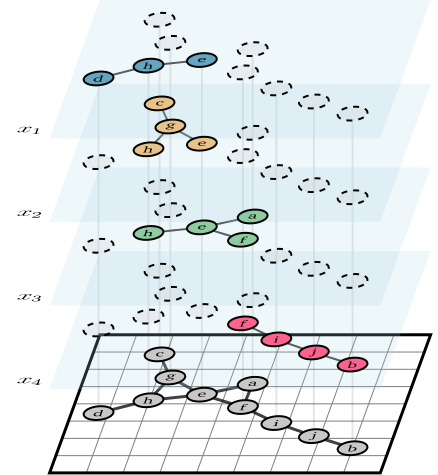
\includegraphics[keepaspectratio]{index_files/mediabag/content/part2/2-02-forest-pursuit_files/figure-latex/..-codefigs-graphs-fig-stack-tree-output-1.pdf}}

}

\caption{\label{fig-stack-tree}Edge Measurements with true (tree)
dependencies known}

\end{figure}%

With the overt link from spreading processes to counts of trees made,
there's room for a more intuitive bridge.

For single-cause, single source spreading process activations---on a
graph---the activation dependency graph for each
observation/spread/random walk \emph{must be a tree}. With a single
cause (the ``root''), which is the starting position of a random walker,
a node can only be reached (activated) by another currently activated
node. If the random walk jumps from one visited node to another,
previously visited one, that transition did not result in an activation
, so the \emph{dependency} count for that edge should not increase. This
description of a random walk, where subsequent visits do not ``store''
the incoming transition, is roughly equivalent to one more commonly
described as a \emph{Loop-Erased} random walk. It is precisely used to
uniformly sample the space of spanning trees on a
graph.\autocite{Generatingrandomspanning_Wilson1996}

Much like a reluctant co-author ``worn down'' by multiple requests, we
can even include random walks that ``receive'' activation potential from
more than one source. Say a node is activated when some fraction of its
neighbors have all originated a random walk transition to it, or a node
activates on its second visit, or similar. We simply count (as
dependency evidence) the ultimate transition that precipitated
activation. This could be justified from an empirical perspective as
well: say we observe an author turn down requests for one paper from two
individuals, but accept a third. We could actually infer a
\emph{lowered} dependency on the first two, \emph{despite} the eventual
coauthorship. Only the interaction that was observed as successful
necessarily counts toward success-dependency, barring any contradicting
information.

It's important to add here that \emph{mutual convincing} by multiple
collaborators simultaneously (or over time) is expressly left out. In
other words, only pairwise interactions are permitted. This is not an
additional assumption, but a key limitation of our use of graphs in the
first place! As Torres et al.~go to great lengths elaborating in
\autocite{WhyHowWhen_Torres2021}, it is critical to correctly model
dependencies when selecting a structural representation of our problem
to avoid data loss. The possibility for multi-way interactions would
necessitate the use of either a simplicial complex or a hypergraph as
the carrier structure, \emph{not a graph}.

Figure~\ref{fig-stack-tree} demonstrates the use of trees as the
distribution for subgraphs, instead of outer-products/cliques.

\section{Sparse Approximation}\label{sparse-approximation}

As indicated previously, we desire a representation of each observation
that takes the ``node space'' vectors (\(\mathbf{x}_i\)) to ``edge
space'' ones (\(\mathbf{r}_i\)). We have separated each observation with
the intention of finding a point-estimate for the ``best'' edges, such
that the edge vector induces a subgraph belonging to a desired class. If
we assume that each edge vector is in \(\mathbb{B}^{\omega}\), so that
the interactions are unweighted, undirected, simple graphs, then for any
family of subgraphs we will be selecting from at most
\(\omega\leq {n\choose 2}\) edges.

Representing a vector as sparse combination of a known set of vectors
(also known as ``atoms'') is called \emph{sparse approximation}.

\subsection{Problem Specification}\label{problem-specification}

Sparse approximation of a vector \(\mathbf{x}\) as a representation
\(\mathbf{r}\) using a dictionary of atoms (columns of \(D\)) is
specified more concretely as
\autocite{EfficientimplementationK_Rubinstein2008}:
\begin{equation}\phantomsection\label{eq-sparse-approx}{\mathbf{\hat{r}} = \operatorname*{argmin}_{\mathbf{r}}{\|\mathbf{x}-D\mathbf{r} \|_2^2} \quad \text{s.t.} \|\mathbf{r}\|_0\leq N }\end{equation}
where \(N\) serves as a sparsity constraint (at most \(N\) non-zero
entries). This is known to be NP-hard, though a number of efficient
methods to approximate a solution are well-studies and widely used.
Solving the lagrangian form of Equation~\ref{eq-sparse-approx}, with an
\(\ell_1\)-norm in place of \(\ell_0\), is known as \_Basis
Pursuit\autocite{SparseApproximateSolutions_Natarajan1995}, while
greedily solving for the non-zeros of \(\mathbf{r}\) one-at-a-time is
called \emph{matching
pursuit}\autocite{Matchingpursuitstime_Mallat1993}. In that work, each
iteration selects the atom with the largest inner product
\(\langle \mathbf{d}_{i'},\mathbf{x}\rangle\).

We take an approach similar to this, but with the insight that the inner
product will not result in desired sparsity (namely, a tree). Our
dictionary in this case will be the set of edges given by \(B\) (see
Section~\ref{sec-subgraph-dists}), while our sparsity is given by the
relationship of the numbers of nodes and edges in a tree:
\begin{equation}\phantomsection\label{eq-sparse-approx-tree}{
\mathbf{\hat{r}} = \operatorname*{argmin}_{\mathbf{r}}{\|\mathbf{x}-B^T\mathbf{r} \|_2^2} \quad \text{s.t.} \|\mathbf{r}\|_0\leq \|\mathbf{x}\|_0 - 1
}\end{equation}

There are some oddities to take into account here. As a linear operator
(see Section~\ref{sec-lin-ops}), \(B^T\) takes a vector of edges to
node-space, counting the number of edges each node was incident to. This
means that, even with a ground-truth set of interactions, \(B^T\) would
take them to a new matrix
\(X_{\text{deg}}(i,j):I\times J \rightarrow \mathbb{N}\), which has
entries of the number of interactions each individual in observation
\(i\) was involved in. While very useful for downstream analysis (see
Section~\ref{sec-fp-preprocess}), the MSE loss in
Equation~\ref{eq-sparse-approx-tree} will never be zero, since
\(X_{\text{deg}}\) entries are not boolean. Large-degree ``hub'' nodes
in the true graph would give a large residual, and the adjoint would
subsequently fail to remove the effect of \(B^T\) on the edge vectors.

It might be possible to utilize a specific semiring, such as
\((\min,+)\), to enforce inner products (see Section~\ref{sec-products})
that take us back to a binary vector.\footnote{ This is more than a
  simple hack, and belies a great depth of possible connection to the
  problem at hand. It is known that ``lines'' (arising from equations of
  the inner product) in tropical projective space \emph{are
  trees}.\autocite{tropicalGrassmannian_2004} In addition, the tropical
  equivalent to Kirchoff's polynomial (which counts over all possible
  spanning trees), is the direct computation of the minimum spanning
  tree.\autocite{TropicalKirchhoffsformula_Jukna2021} For treatment of
  sparse approximation using tropical matrix factorization, see
  \textcite{Sparsedataembedding_Omanovic2021}} Instead, we will take an
empirical bayes approach to the estimation of sparse
vectors.\autocite{EmpiricalBayesianStrategy_Wipf2007} As a probabilistic
graphical model, we assume each observation is emitted from a
(tree-structured) MRF {[}explained?{]} on the activated nodes. This is
underdetermined (any spanning tree could equally emit the observed
activations), so we use an empirical prior as a form of shrinkage: the
co-occurrences of nodes across all observed activation patterns. This
let's us optimize a likelihood from Equation~\ref{eq-edgevec-prob}, for
the distribution of spanning trees on the subgraph of \(G^*\) inducted
by \(\mathbf{x}\).
\begin{equation}\phantomsection\label{eq-sparse-approx-tree}{
\mathbf{\hat{r}} = \operatorname*{argmax}_{\mathbf{r}}{\mathcal{L}(\mathbf{r}|\mathbf{x})} \quad \text{s.t.}\quad \mathbf{r}\sim \mathcal{T}(G^*[\mathbf{x}])
}\end{equation}

\subsection{Max. Spanning (Steiner)
Trees}\label{max.-spanning-steiner-trees}

The point estimate \(\hat{\mathbf{r}}\) is therefore the mode of a
distribution over trees, which is precisely the maximum spanning
tree.\autocite{EfficientComputationExpectations_Zmigrod2021} If we allow
the use of all observations \(X\) to find an empirical prior for
\(\mathbf{r}\), then we can calculate a value for the mutual information
for the activated nodes, and use this to directly calculate the Chow-Liu
estimate. One algorithm for finding a maximum spanning tree is
Prim's{[}CITE?{]}, which effectively performs the matching pursuit
technique of greedily adding an edge (i.e.~non-zero entry in our vector)
one-by-one. In this way, we effectively \emph{do} perform matching
pursuit, but minimizing the KL-divergence between observed node
activations and a tree-structured MRF limited to those nodes, alone
(rather than the mean-square-error).

However, the mode of the tree distribution is not strictly the one that
uses mutual information as edge weights. There is reason to believe that
edge weights based on pairwise joint probabilities might also be
appropriate. Namely, the Hunter-Worsley bound for unions of (dependent)
variables says that the sum of marginal probabilities over-counts the
true union of activations (including by dependence relations). This
alone would be known as Boole's inequality, but the amount it overcounts
is \emph{at most} the weight of the maximum spanning tree over pairwise
joint probabilities.\autocite{upperboundprobability_Hunter1976} Adding
the tree of joint co-occurrence probabilities is the most conservative
way to arrive at the observed marginals from the probability of at least
one node occurring (which could then be the ``root'').

Finally, we realize that the problem statement (``find the maximum
weight tree on the subgraph'') is not the same as an MST, per-se, but
rather the so-called ``Steiner Tree'' problem. In other words, we would
like our tree of interactions to be of minimum weight on a node-induced
subgraph \emph{of the true graph}. The distribution of trees that our
interactions are sampled from should be over the available edges in the
recovered graph, \emph{which we do not yet have}. Thankfully, a
well-known algorithm for approximating the (graph) Steiner tree problem
instead finds the minimum spanning tree over the \emph{metric closure}
of the graph.\autocite{fastalgorithmSteiner_Kou1981}

This metric closure is a complete graph having weights given by the
shortest-path distances between nodes. While we don't know those exact
values either, we do have the fact that the distance metric implied by
the forest kernel (in Equation~\ref{eq-regulap}) is something of a
relaxation of shortest paths. In the limit \(\beta\rightarrow 0\), \(Q\)
is proportional to shortest path distances, while
\(\beta\rightarrow\infty\) instead gives commute/resistance
distances.\autocite{Semisupervisedlearning_Avrachenkov2017} And that
kernel is counting the probability of co-occurrence on trees in any
random spanning forest!

All this is to say that node co-occurrence measures are more similar to
node-node distances in the underlying graph, \emph{not estimators of
edge existence}. But we can use this as an empirical prior to
approximate Steiner trees that \emph{are on the true graph}.

\section{Forest Pursuit}\label{sec-FP}

Instantiating the above, we propose \emph{Forest Pursuit}, an relatively
simple algorithm for correction of clique-bias under a spreading process
assumption

\subsection{Algorithm Summary}\label{algorithm-summary}

Once again, we assume \(m\) observations of activations over \(n\)
nodes, represented as the design matrix
\(X:I\times J \rightarrow \mathbb{B}\). Like GLASSO, we assume that a
Gram matrix (or re-scaling of it) is precomputed, for the non-streaming
case.

Based on the discussion in Tip~\ref{tip-cs} we will use the cosine
similarity as a degree-corrected co-occurrence measure, with node-node
distances estimated as \(d_K=-\log{\text{Ochiai}(j,j')}\).\footnote{
  Note that any kernel could be used, given other justification, though
  anecdotal evidence has the negative-log-Ochiai distance performing
  marginally better than MI distance or Yule's \(Q\).}

For each observation, the provided distances serve to approximate the
metric closure of the underlying subgraph induced by \(\mathbf{x}\).
This is passed to an algorithm for finding the minimum spanning tree.
Given a metric closure, the MST in turn would be an approximation of the
desired Steiner tree within \(2-\tfrac{2}{\|\mathbf{x}\|_0}\) of
optimal.\autocite{fastalgorithmSteiner_Kou1981} For
\(\|\mathbf{x}\|_0 \ll n\), this error bound will often be close to 1,
and approaching 2 as the expected number of activations-per-observation
grows.

After the point estimates for \(\mathbf{r}\) have been calculated as
trees, we can use the desire-path beta-binomial model
(Equation~\ref{eq-desirepath-binom}) to calculate the overall empirical
Bayes estimate for \(\hat{G}\). As a prior for \(\alpha\), instead of a
Jeffrey's or Laplace prior, we bias the network toward maximal sparsity,
while still retaining connectivity. In other words, we assume that \(n\)
nodes only need about \(n-1\) edges to be fully connected, which implies
a prior expected sparsity of
\begin{equation}\phantomsection\label{eq-min-connect}{
\alpha^*=\frac{n-1}{\tfrac{1}{2}n(n-1)} = \frac{2}{n}
}\end{equation} which we can use as a sparsity-promoting initial value
for \(\text{Beta}(\alpha^*,1-\alpha^*)\).

\begin{algorithm}[htb!]
\caption{Forest Pursuit}
\label{alg-fp}
\begin{algorithmic}[1]
\Require $X\in \mathbb{B}^{m\times n}, d_K\in \mathbb{R}_{\geq 0}^{n\times n}, 0<\alpha<1$
\Ensure $R \in \mathbb{B}^{m \times {n\choose 2}}$
\Procedure{ForestPursuitEdgeProb}{$X, d_K, \alpha$}
  \State $R \gets $\Call{ForestPursuit}{$X, d_K$}
  \State $\hat{\alpha}_m\gets$\Call{DesirePathBeta}{$X,R, \alpha$}
  \State \textbf{return} $\hat{\alpha}_m$
\EndProcedure
\Procedure{ForestPursuit}{$X, d_K$}
  \State $R(\cdot,\cdot) \gets 0$
  \For{$i\gets 1, m$}\Comment{\textit{each observation}}
    \State $\mathbf{x}_i \gets X(i,\cdot)$
    \State $R(i,\cdot) \gets $\Call{PursueTree}{$\mathbf{x}_i, d_K$} 
  \EndFor
  \State \textbf{return} $R$
\EndProcedure
\Procedure{PursueTree}{$\mathbf{x}, d$}
\Comment{\textit{Approximate Steiner Tree}}
  \State $V \gets \{v\in \mathcal{V} | \mathbf{x}(\mathcal{V})=1\}$
  \Comment{\textit{activated nodes}}
  \State $T \gets$\Call{MST}{$d[V,V]$}
  \Comment{\textit{e.g. Prim's Algorithm}}
  \State $\mathbf{u,v}\gets \{(j,j')\in J\times J | T(j,j')\neq 0\}$
  \State $\mathbf{r} \gets e_n(\mathbf{u,v})$
  \Comment{\textit{unroll tree adjacency}}
  \State \textbf{return} $\mathbf{r}$ 
\EndProcedure
\Procedure{DesirePathBeta}{$X,R, \alpha$}
  \State $\mathbf{s} \gets \sum_{i=1}^m R(i,e)$
  \State $\sigma \gets \sum_{i=1}^m X(i,j)$
  \State $\mathbf{k} \gets e_n(\sigma\sigma^T)$
  \Comment{\textit{co-occurrence counts}}
  \State $\hat{\alpha}_m \gets \alpha + \frac{\mathbf{s}-\alpha \mathbf{k}}{\mathbf{k}+1}$
  \State \textbf{return} $\hat{\alpha}_m$
\EndProcedure
\end{algorithmic}
\end{algorithm}

Algorithm~\ref{alg-fp} outlines the algorithm in pseudocode for
reproducibility.

\subsection{Approximate Complexity}\label{sec-fp-complexity}

The Forest Pursuit calculation presented in Algorithm~\ref{alg-fp}
assumes an initial value for the distance matrix, which is similar to
the covariance estimate that is pre-computed (as an initial guess) for
GLASSO. Therefore we do not include the matrix multiplication for the
gram matrix in our analysis, at least in the non-streaming case. Because
every observation is dealt with completely independently, the FP
estimation of \(R\) is linear in observation count. It is also trivially
parallelizeable,\footnote{Although, no common python implementation of
  MST algorithms are as-yet vectorized or parallelized for simultaneous
  application over many observations. We see development of non-blocking
  MSTs in common analysis frameworks as important future work.} and the
bayesian update for \(\hat{\alpha}_m\) can be performed in a streaming
manner, as well.

Each observation requires a call to ``PursueTree'', which involves an
MST call for the pre-computed subset of distances onnodes activated for
that observation. Note the use of MST algorithm could apply Prim's or Kr
uskal's algorithm, or similar. It is recommended to utilize Prims in
this case, however, since Prim's on a sufficiently dense graph can be
made to run in \(O(n)\) time for \(n\) activated nodes by using a
\emph{d}-tree for its heap queue.{[}CITE{]} Since we are always using
the metric closure, Prim's will always run on a complete graph.

Importantly, this means that FP does not scale with the the size of the
network, but only the worst-case activation count of a given
observation, \(O(s_{\text{max}})\), where
\(s_{\text{max}}=\max_i{(\|X(i,\cdot)\|_0)}\) We say this is
\emph{approximately} constant in node size:

\begin{itemize}
\tightlist
\item
  the total number of nodes is typically a \emph{given} for a single
  problem setting
\item
  in many domains, the basic \emph{spreading} rate of diffusion model
  (e.g.~\(R_0\), or heat conductivity), does not scale with the total
  size of an observation
\end{itemize}

That last point means that constant scaling with network size is
generally down to the domain in question. For instance, a heat equation
simulated over a small area, having a given conductivity, will not have
a different conductivity over a larger area; conductivity is a material
property. Similarly, a virus might have a particular basic reproduction
rate, or a set of authors might have a static distribution over how many
collaborators they wish to work with. The former is down to viral load
generation, and the latter a sociological limit: more a bigger
department usually doesnt imply more co-authors.

Similar to Equation~\ref{eq-min-connect}, we might reasonably assume
that the expected degree of nodes is roughly constant with network size
i.e.~a property of domain. So, the the density of activation vectors (as
a fraction of all possible edges) is going go scale with the inverse of
\(n\). This makes a process linear in activation count to be constant in
network size. Then, if \(\bar{s}\) is the expected non-zero count of
each row of \(X\), the final approximate complexity of FP is
\(O(m\bar{s})\).\footnote{ In our reference implementation, which uses
  Kruskal's algorithm, the theoretical complexity is likewise
  \(O(m\bar{s}^2\log{\bar{s}})\), though in our experience the values of
  \(\bar{s}\) are small enough to not impact the runtime significantly.}

\section{Simulation Study}\label{sec-FP-experiments}

To test the performance of FP against other backboning and recovery
methods, we have developed a public repository
\href{https://github.com/rtbs-dev/affinis}{\texttt{affinis}} containing
reference implementations for FP, along with many co-occurrence and
backboning techniques. The library contains source code and examples for
many of the presented methods, and more. {[}UPDATE w/ DOI?{]}

In addition, to support the community and provide for a standard set of
benchmarks for network recovery from activations, the
\href{https://github.com/rtbs-dev/mendr}{\texttt{MENDR}} reference
dataset and testbench was developed. To make reproducible comparison of
recovery algorithms easier, \texttt{MENDR} includes hundreds of randomly
generated networks in several classes, along with random walks sampled
\emph{on those networks}. It can also be extended through community
contribution, using data versioning to allow consistent comparison
between different reports and publications over time.

\subsection{Experimental Method}\label{experimental-method}

For each algorithm shown in Table~\ref{tbl-methods}, every combination
of the parameters in Table~\ref{tbl-mendr} was tested. 30 random graphs
for each of nodes were tested, which was repeated again for each of
Tree, Block, and scale-free types.

\begin{longtable}[]{@{}
  >{\raggedright\arraybackslash}p{(\linewidth - 2\tabcolsep) * \real{0.2500}}
  >{\centering\arraybackslash}p{(\linewidth - 2\tabcolsep) * \real{0.7500}}@{}}
\caption{Experiment Settings (MENDR
Dataset)}\label{tbl-mendr}\tabularnewline
\toprule\noalign{}
\begin{minipage}[b]{\linewidth}\raggedright
parameters
\end{minipage} & \begin{minipage}[b]{\linewidth}\centering
values
\end{minipage} \\
\midrule\noalign{}
\endfirsthead
\toprule\noalign{}
\begin{minipage}[b]{\linewidth}\raggedright
parameters
\end{minipage} & \begin{minipage}[b]{\linewidth}\centering
values
\end{minipage} \\
\midrule\noalign{}
\endhead
\bottomrule\noalign{}
\endlastfoot
random graph \textbf{kind} & Tree, Block, BA\((m\in\{1,2\}\)) \\
network \textbf{\(n\)-nodes} & 10,30,100,300 \\
random \textbf{walks} & 1 sample
\(m\sim\text{NegBinomial}(2,n^{-1})+10\) \\
random walk \textbf{jumps} & 1 sample
\(n_\sim\text{Geometric}(n^{-1})+5\) \\
random walk \textbf{root} & 1 sample
\(n_0 \sim \text{Multinomial}(\textbf{n}^{-1},1)\) \\
random \textbf{seed} & 1, 2, \ldots{} , 30 \\
\end{longtable}

\begin{longtable}[]{@{}
  >{\raggedright\arraybackslash}p{(\linewidth - 8\tabcolsep) * \real{0.3729}}
  >{\centering\arraybackslash}p{(\linewidth - 8\tabcolsep) * \real{0.1525}}
  >{\centering\arraybackslash}p{(\linewidth - 8\tabcolsep) * \real{0.1695}}
  >{\centering\arraybackslash}p{(\linewidth - 8\tabcolsep) * \real{0.1695}}
  >{\raggedleft\arraybackslash}p{(\linewidth - 8\tabcolsep) * \real{0.1356}}@{}}
\caption{Summary of algorithms
compared}\label{tbl-methods}\tabularnewline
\toprule\noalign{}
\begin{minipage}[b]{\linewidth}\raggedright
Algorithm
\end{minipage} & \begin{minipage}[b]{\linewidth}\centering
abbrev.
\end{minipage} & \begin{minipage}[b]{\linewidth}\centering
\(\alpha\)?
\end{minipage} & \begin{minipage}[b]{\linewidth}\centering
class
\end{minipage} & \begin{minipage}[b]{\linewidth}\raggedleft
source
\end{minipage} \\
\midrule\noalign{}
\endfirsthead
\toprule\noalign{}
\begin{minipage}[b]{\linewidth}\raggedright
Algorithm
\end{minipage} & \begin{minipage}[b]{\linewidth}\centering
abbrev.
\end{minipage} & \begin{minipage}[b]{\linewidth}\centering
\(\alpha\)?
\end{minipage} & \begin{minipage}[b]{\linewidth}\centering
class
\end{minipage} & \begin{minipage}[b]{\linewidth}\raggedleft
source
\end{minipage} \\
\midrule\noalign{}
\endhead
\bottomrule\noalign{}
\endlastfoot
Forest Pursuit & FP & Yes & hybrid & - \\
GLASSO & GL & No & MRF &
\autocite{Sparseinversecovariance_Friedman2008,Structureestimationdiscrete_Loh2012} \\
Ochiai Coef. & CS & Yes & Counts &
\autocite{Measuresecologicalassociation_Janson1981} \\
Hyperbolic Projection & HYP & No & Counts &
\autocite{Scientificcollaborationnetworks._Newman2001} \\
Doubly-Stochastic & eOT & Yes & Transport &
\autocite{twostagealgorithm_Slater2009,Sinkhorndistanceslightspeed_Cuturi2013} \\
High-Salience Skeleton & HSS & Yes & Transport &
\autocite{Robustclassificationsalient_Grady2012} \\
Resource Allocation & RP & Yes & Transport &
\autocite{Bipartitenetworkprojection_Zhou2007} \\
\end{longtable}

For each algorithm that could be supplied a prior via additive
smoothing, seen in Table~\ref{tbl-methods} as ``\(\alpha\)?: Yes'', a
minimum connected (tree) level of sparsity wasy supplied
\(\alpha=\tfrac{2}{n}\). The others, esp.~GLASSO, do not have a
\(\tfrac{\text{count}}{\text{exposure}}\) form, and could not be easily
interpreted in a way that allowed for additive smoothing. However, since
the regularizaiton parameter for GLASSO is often critical for finding
good solutions, a 5-fold cross validation was performed for each
experiment to select a ``best'' value, with the final result run using
that value. While this does have a constant-time penalty for each
experiment, the reconstruction accuracy is significantly improved with
this technique, and would reflect common practice in using GLASSO for
this reason.

The three classes of random graphs represent common use cases in sparse
graph recovery. In addition, the block and tree graphs are types we
expect GLASSO to correctly recover in this binary
setting.\autocite{Structureestimationdiscrete_Loh2012} The block graphs
of size \(n\) were formed by taking the line-graph of randomly generated
trees of size \(n+1\).\\
Trees were randomly generated using Prüfer sequences as impelmented in
NetworkX {[}CITE{]}. To simulate possible social networks and other
complex systems that show evidence of preferential attachment,
scale-free graphs were sampled through the Barabási--Albert (BA) model,
which was randomly seeded with a re-attachment paramenter \(m\) of
either 1 or 2.

Every graph has a static ID provided by MENDR, along with generation and
retrieval code for public review. New graphs kinds and sizes are simple
to add for future benchmarking capability.

\subsection{Metrics}\label{metrics}

To compare each algorithm consistently, several performance measures
have been included in the MENDR testbench. They are all functions of the
True Positive/Negative (TP/TN) and False Positive/Negative (FP/FN)
values.

\begin{description}
\tightlist
\item[Precision (P)]
Fraction of positive predictions that are true, also called ``positive
predictive value'' (PPV) \[P= \frac{TP}{TP+FP}\]
\item[Recall (R)]
Fraction of true values that were returned as positive. Also called the
TP-rate (TPR), and has an inherent trade-off with precision.
\[R=\frac{TP}{TP+FN} \]
\item[Matthews Correlation Coefficient (MCC)]
Balances all of TP,TN,FP,FN. Preferred for class-imbalanced problems
(like sparse recovery)
\autocite{statisticalcomparisonMatthews_Chicco2023}
\[\frac{TP\cdot TN - FP\cdot FN}{\sqrt{(TP+FP)(TP+FN)(TN+FP)(TN+FN)}}\]
\item[Fowlkes-Mallows (F-M)]
Geometric mean of Precision and Recall, as opposed to the F-Measure that
returns the harmonic mean. Also known to be the limit of the MCC as TN
approaches infinity\autocite{MCCapproachesgeometric_Crall2023}, which is
useful as TN grows with \(n^2\) but TP only with \(n\).
\[\sqrt{P\cdot R}\]
\end{description}

Because this work is focused on unsupervised performance, specifically
for the use of these algorithms by analysts investigating dependencies,
we opt to calculate TP,TN,FP,FN at every unique edge
probability/strength value returned by each algorithm. Then, because we
do not know a priori which threshold level will be selected by an
analyst in the unsupervised setting, we take a conservative approach and
report the expected values E{[}MCC{]} and E{[}F-M{]} over all unique
threshold values. To consistently compare the expected values, we
transform the thresholds for every experiment to the range
\([\epsilon, 1-\epsilon]\), to avoid division-by-0 at the extremes.

Another common approach is to report the Average Precision Score (APS).
This is not the average precision over the thresholds however, but
instead the expected precision over the possible recall values
achievable by the algorithm. It is approximating the integral under the
parametric P-R curve, instead of the thresholds themselves.
\[\text{APS} = \sum_{e=1}^{\omega} P(e)(R(e)-R(e-1))\] where \(P(e)\)
and \(R(e)\) are the precision and recall at the threshold set by the
edge \(e\), in rank-order. This is more commonly done for supervised
settings, however, and will report a high value as long as \emph{any}
threshold is able to return a both a high precision and a high recall,
simultaneously.

\subsection{Results - Scoring}\label{results---scoring}

The results over every experiment are shown in
Figure~\ref{fig-fp-overall}. Only FP is able to report MCC and F-M
values with medians over about 0.5, regularly reaching over 0.8. GLASSO
is clearly the second-best at recovery in these experiments, though for
scale-free networks the improvement over simply thresholding the Ochiai
coefficient is negligible. For APS, both GLASSO and Ochiai are equally
able to return high scores, indicating at least one threshold for each
that performed well. A simple mechanism for FP to perform equally well
at APS is discussed in Section~\ref{sec-fpi}.

\begin{figure}

\centering{

\pandocbounded{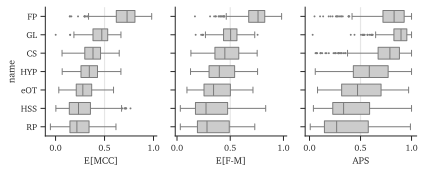
\includegraphics[keepaspectratio]{index_files/mediabag/content/part2/2-02-forest-pursuit_files/figure-latex/..-codefigs-results-fig-fp-overall-output-1.pdf}}

}

\caption{\label{fig-fp-overall}Comparison of MENDR recovery scores}

\end{figure}%

Breaking down the results by graph kind in Figure~\ref{fig-fp-compare},
we see the remarkable ability of FP to dramatically outperform every
other algorithm in MCC and F-M, showing remarkable accuracy
\emph{together with stability} over the set of threshold values. This is
indicative of FP's ability to more directly estimate the support of each
edge, with lower values occurring only when co-occurrences aren't being
consistently explained with the same set of incidences.

\begin{figure}

\centering{

\pandocbounded{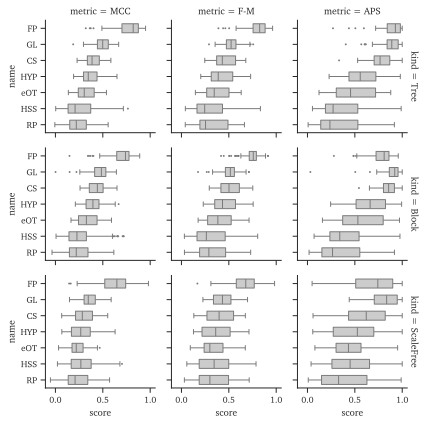
\includegraphics[keepaspectratio]{index_files/mediabag/content/part2/2-02-forest-pursuit_files/figure-latex/..-codefigs-results-fig-fp-compare-output-1.pdf}}

}

\caption{\label{fig-fp-compare}Comparison of MENDR Recovery Scores by
Graph Type}

\end{figure}%

Another important capability of any recovery algorithm is to improve its
estimate when provided with more data. Of course, this also will depend
on other factors, such as the dimensionality of the problem (network
size), and specifically for us, whether \emph{longer} random walks makes
network inference better or worse.

\begin{figure}

\centering{

\centering{

\pandocbounded{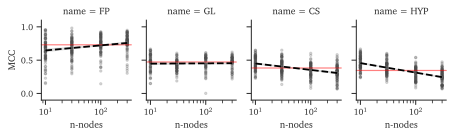
\includegraphics[keepaspectratio]{index_files/mediabag/content/part2/2-02-forest-pursuit_files/figure-latex/..-codefigs-results-fig-mendr-trends-output-1.pdf}}

}

\subcaption{\label{fig-mendr-trends-1}Trend: MCC vs network size}

\centering{

\pandocbounded{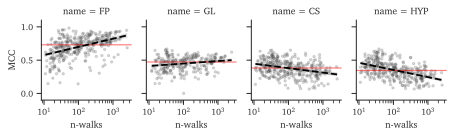
\includegraphics[keepaspectratio]{index_files/mediabag/content/part2/2-02-forest-pursuit_files/figure-latex/..-codefigs-results-fig-mendr-trends-output-2.pdf}}

}

\subcaption{\label{fig-mendr-trends-2}Trend: MCC vs observation count}

\centering{

\pandocbounded{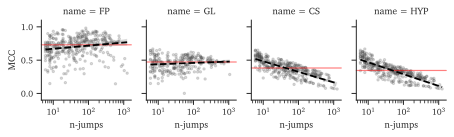
\includegraphics[keepaspectratio]{index_files/mediabag/content/part2/2-02-forest-pursuit_files/figure-latex/..-codefigs-results-fig-mendr-trends-output-3.pdf}}

}

\subcaption{\label{fig-mendr-trends-3}Trend: MCC vs random-walk length}

}

\caption{\label{fig-mendr-trends}Score trends vs problem scaling}

\end{figure}%

As Figure~\ref{fig-mendr-trends} shows, FP is positively correlated with
\emph{all three}. Most importantly, the trend for FP is strongest as the
number of observations increases, which is not a phenomenon seen in the
other methods. In fact, it appears that count-based methods' scores are
negatively correlated with added random walk length and added
observations. Only HYP and CS scores are shown in
Figure~\ref{fig-mendr-trends}, but all other tested methods (other than
FP and GLASSO) show the same trend.

However, because the graph sampling protocol includes \(n\) in the
distributions for the observation count and random-walk length, we
additionally performed a linear regression on the (log) parameters. The
\emph{partial resitual} plots are shown in
Figure~\ref{fig-partials-mcc}, which shows the trends of each variable
after controlling for the others.

\begin{figure}

\centering{

\pandocbounded{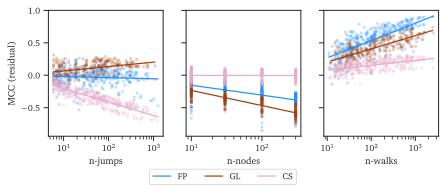
\includegraphics[keepaspectratio]{index_files/mediabag/content/part2/2-02-forest-pursuit_files/figure-latex/..-codefigs-results-fig-partials-mcc-output-1.pdf}}

}

\caption{\label{fig-partials-mcc}Partial Residuals (regression on
E{[}MCC{]})}

\end{figure}%

This analysis indicates that \emph{all} methods should likely increase
in their performance when extra observations are added, though FP does
this more efficiently than either CS or GLASSO. Interestingly, CS is
largely unaffected by network size, compared to FP and GL, though GL
performs the worst in this regard. However, it is in the random-walk
length that we see the benefit of dependency-based algorithms. The
Ochiai coefficient suffers dramatically as more nodes are activated by
the spreading process, since this means the implied clique size grows by
the square of the number of activations. FP remains unaffected by
walk-length, while (impressively) GLASSO appears to have a marginal
boost in performance when walk lengths are high.

\subsection{Results - Runtime
Performance}\label{results---runtime-performance}

For both Forest Pursuit and GLASSO, runtime efficiency is critical if
these algorithms are going to be adopted by analysts for backboning and
recovery. Figure~\ref{fig-runtime} shows the (log-)seconds against the
same parameters from before. For similar sized networks, FP is
consistently taking 10-100x less time to reach a result than GLASSO
does. Additionally, many of the experiments led to ill-conditioned
matrices that failed to converge for GLASSO under any of the
regularization parameters tests (the ``x'' markers in
Figure~\ref{fig-runtime}). As expected, the number of observations plot
shows a clear limit in terms of controlling the lower-bound of FPs
runtime, since in this serial version every observation runs one more
call to MST. On the other hand, GLASSO appears to have signiicant
banding for walk length and observation counts, likely indicating
dominance of network size for its runtime.

\begin{figure}

\centering{

\pandocbounded{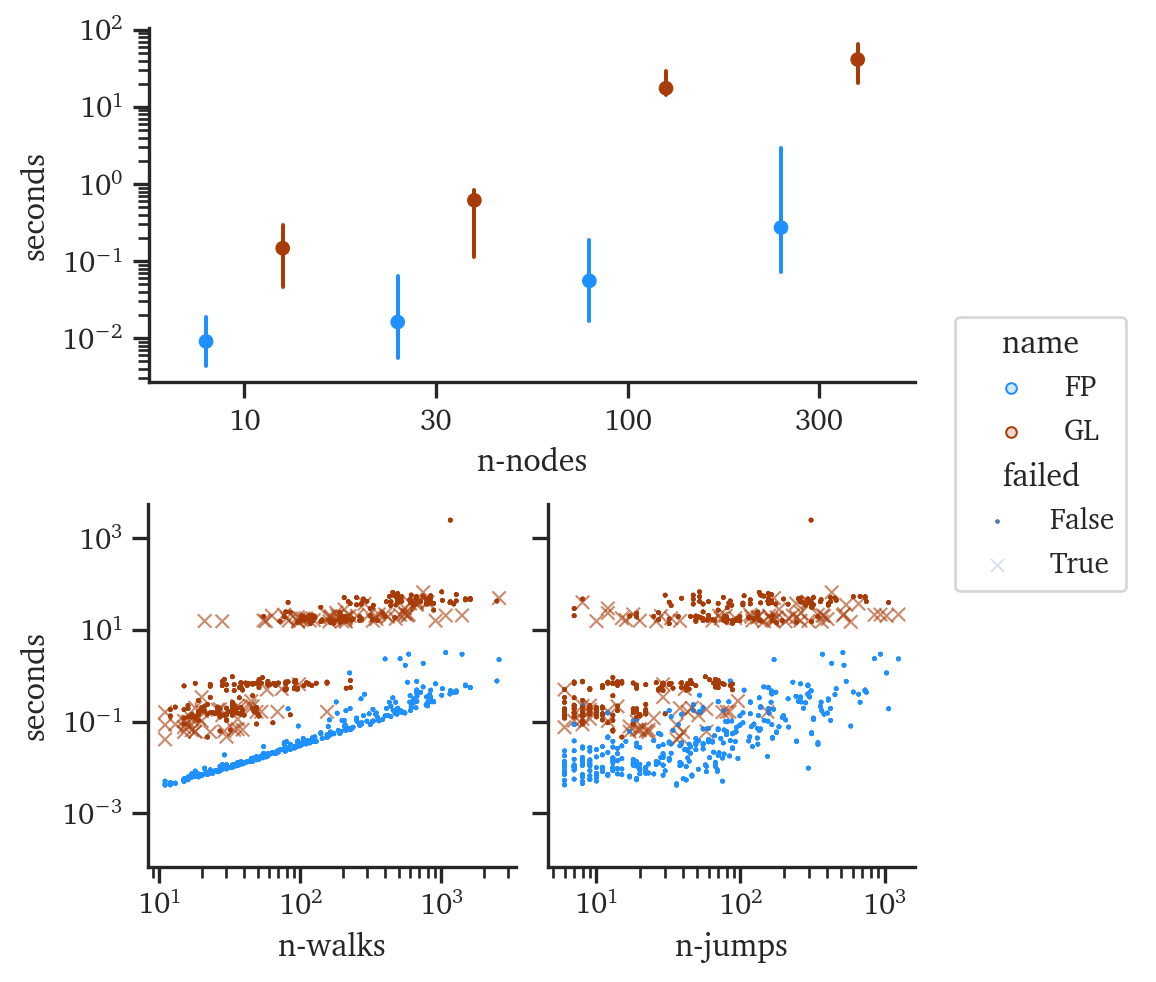
\includegraphics[keepaspectratio]{content/part2/2-02-forest-pursuit_files/figure-latex/..-codefigs-results-fig-runtime-output-1.png}}

}

\caption{\label{fig-runtime}Runtime Scaling (Forest-Pursuit vs GLASSO)}

\end{figure}%

To control for each of the variables, and to empirically validate the
theoretical analysis in Section~\ref{sec-fp-complexity}\}, a regression
of the same three (log-)parametwers was performed against (log-)seconds.
The slopes in Figure~\ref{fig-partials-runtime}, which are plotted on a
log-log scale, correspond roughly to polynomial powers in linear scale.
In regression terms, we are fitting the log of
\[y_{\text{sec}} = ax_{\text{param}}^\gamma\] so that the slope in a
log-log plot is \(\gamma\).

\begin{figure}

\centering{

\pandocbounded{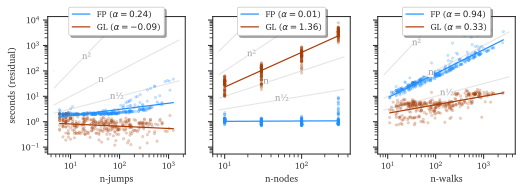
\includegraphics[keepaspectratio]{index_files/mediabag/content/part2/2-02-forest-pursuit_files/figure-latex/..-codefigs-results-fig-partials-runtime-output-1.pdf}}

}

\caption{\label{fig-partials-runtime}Partial Residuals (regression on
computation time)}

\end{figure}%

In a very close match to our previous analysis, the scaling of FP is
almost entirely explained by the observation count and random-walk
length, alone: the coefficient on network size shows constant-time
scaling. Similarly, the scaling with observation count is very nearly
linear time, as predicted. The residuals show non-linear behavior for
the random-walk length parameter, which would make sense, due to the
theoretical \(\|E\|\log\|V\|\) scaling of kruskal's algorithm. At this
scale, \(n\log n\) and \(n^2\log n\) complexity might appear smaller
than linear time, due to the log factor. GLASSO hardly scales with
random walk length, and only marginally with observation count. In
typical GLASSO, the observation count has already been collapsed to
calculate the empirical covariance matrix, so its effects here might be
due instead to the cross-validation and the need to calculate empirical
covariance for observation subsets. The big difference, however, is
GLASSO scaling in significantly superlinear time---almost \(O(n^2)\).
This is usually the limiting factor for analyst use of such an algorithm
in network analysis more generally.

\chapter{Modifications \& Extensions}\label{modifications-extensions}

\section{Forest Pursuit Interaction Probability}\label{sec-fpi}

Without using stability
selection\autocite{StabilitySelection_Meinshausen2010}, GLASSO is not
directly estimating the ``support'' of the edge matrix, but the strength
of each edge. to do similar with FP, we could directly estimate the
frequency of edge occurrence using \(R(i,e)\) marginal averages, rather
than conditioning on co-occurrence. Simply multiplying each FP edge
probability by the co-occurrence probability of each node-node pair
gives this as well, which we call FPi: the direct ``interaction
probability'' for each pair of nodes.

\subsection{Simulation Study
Revisited}\label{simulation-study-revisited}

By doing this simple re-weighting, FPi actually beats GLASSO's median
APS for the dataset, but at the cost of MCC and F-M scores (which both
drop to between FP and GLASSO), as Figure~\ref{fig-fpi} demonstrates.
Similarly, the individual breakdown by graph kind in Table~\ref{tbl-fpi}
shows a similar pattern, with FPi coming close to GLASSO for scale-free
networks, but exceeding it for trees and matching for block graphs.
Still, the difference is small enough, and at such a significant penaly
to MCC and F-M scores over a variety of thresholds, that it is hard to
recommend the FPi re-weighting unless rate-based edge analysis is
desired, e.g.~if Poisson or Exponential occurrence models are desired.

\begin{figure}

\begin{minipage}{0.50\linewidth}

\begin{longtable}[]{@{}llll@{}}

\caption{\label{tbl-fpi}Comparing scores for FP, FPi and GLASSO}

\tabularnewline

\toprule\noalign{}
& FP & FPi & GL \\
\midrule\noalign{}
\endhead
\bottomrule\noalign{}
\endlastfoot
\multicolumn{4}{@{}l@{}}{%
Block} \\
APS & 0.78 & 0.9 & 0.9 \\
F-M & 0.74 & 0.57 & 0.51 \\
MCC & 0.7 & 0.55 & 0.46 \\
\multicolumn{4}{@{}l@{}}{%
ScaleFree} \\
APS & 0.69 & 0.76 & 0.81 \\
F-M & 0.67 & 0.46 & 0.44 \\
MCC & 0.63 & 0.43 & 0.36 \\
\multicolumn{4}{@{}l@{}}{%
Tree} \\
APS & 0.9 & 0.92 & 0.88 \\
F-M & 0.81 & 0.66 & 0.53 \\
MCC & 0.78 & 0.65 & 0.49 \\

\end{longtable}

\end{minipage}%
%
\begin{minipage}{0.50\linewidth}

\begin{figure}[H]

\centering{

\pandocbounded{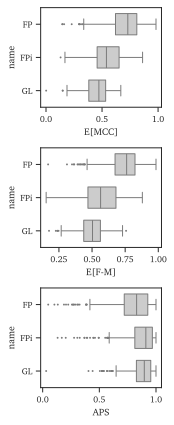
\includegraphics[keepaspectratio]{index_files/mediabag/content/part2/2-03-latent-forest-alloc_files/figure-latex/..-codefigs-results-fig-fpi-output-1.pdf}}

}

\caption{\label{fig-fpi}FPi shows best APS, lower MCC,F-M}

\end{figure}%

\end{minipage}%

\end{figure}%

\subsection{Simulation Case Study}\label{simulation-case-study}

To illustrate what is going on, we have selected two specific
experiments as a case study, in Figure~\ref{fig-pr-curves} In the first,
\texttt{BL-N030S01}, a 30-node block graph with 53 random walk samples,
has FP performing worse than GLASSO and Ochiai, in terms of APS (which
is reported in the legends). We see that FP shows high precision, which
drops off significantly to increase recall at all. Only a few edges had
high probability (which is usually desirable for sparse approximation),
and some of the true edges were missed this way. However, FPi rescaling
makes rarer edges fall off earlier in the thresholding, letting the
recall rise by dropping rare edges, rather than simply the
low-confidence ones.

In the second, \texttt{SC-N300S01} is a 300-node scale-free network with
281 walks. Both FP and FPi show significantly better recovery
capability, since enough walks have visited a variety of nodes to give
FP better edge coverage. In this graph, no algorithm comes within 0.25
of FP's impressive 0.88 APS for 300 nodes fewer than that many walks.

\begin{figure}

\centering{

\pandocbounded{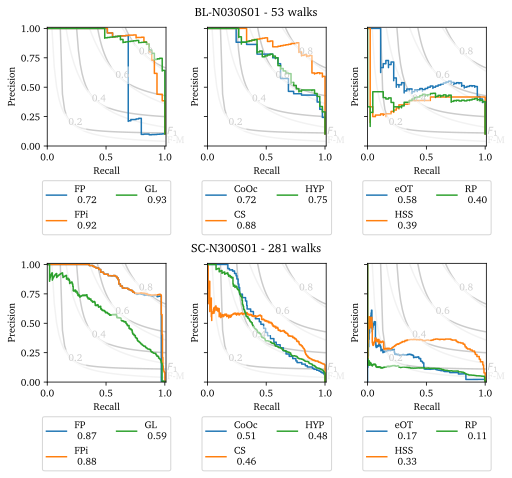
\includegraphics[keepaspectratio]{index_files/mediabag/content/part2/../images/PR.pdf}}

}

\caption{\label{fig-pr-curves}P-R curves for two experiments}

\end{figure}%

\section{Generative Model Specification}\label{sec-lfa-like}

Symmetry of marked directed and undirected trees (symmetry in
\(Q\))\autocite{MatrixForestTheorem_Chebotarev2006}

\begin{figure}

\centering{

\pandocbounded{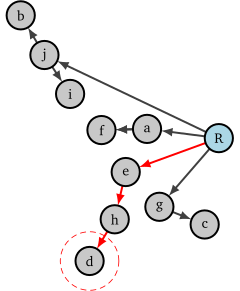
\includegraphics[keepaspectratio]{index_files/mediabag/content/part2/2-03-latent-forest-alloc_files/figure-latex/..-codefigs-graphs-fig-inject-plan-output-1.pdf}}

}

\caption{\label{fig-inject-plan}Dissemination plan as rooted RST on
augmented graph}

\end{figure}%

\pandocbounded{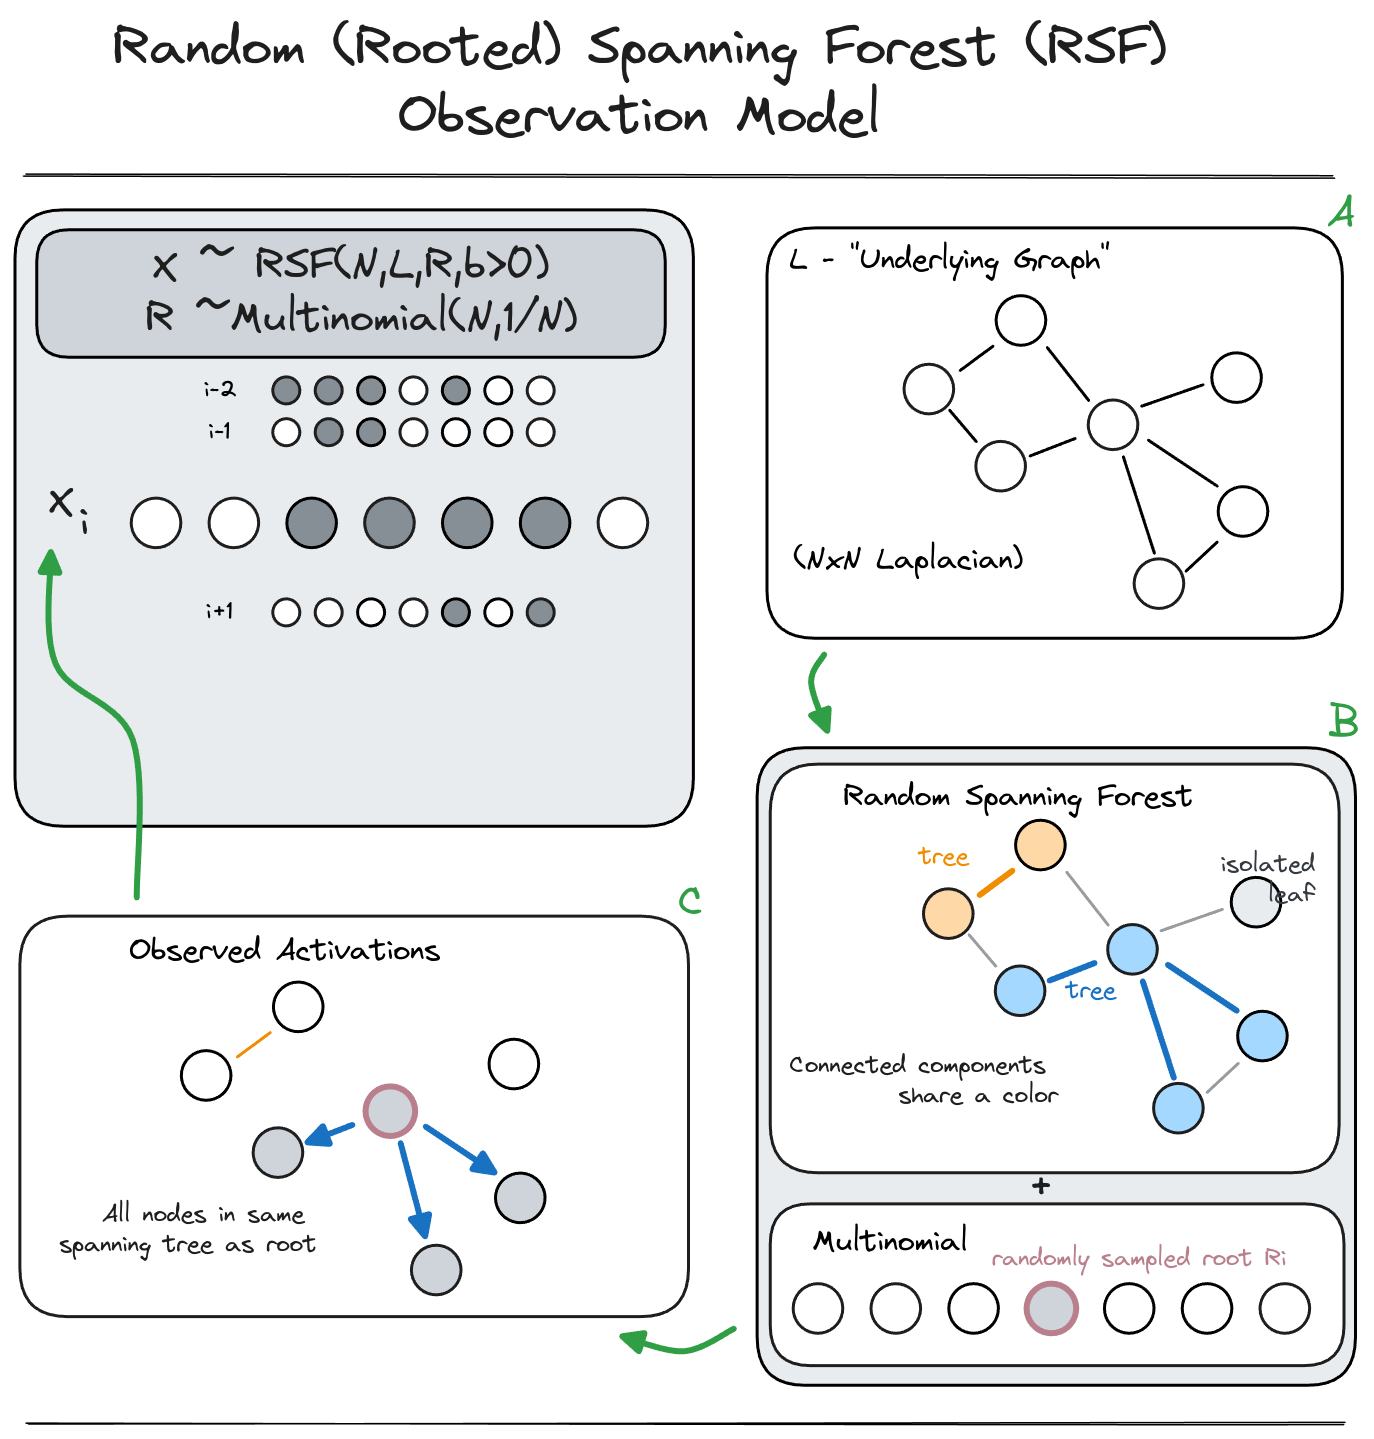
\includegraphics[keepaspectratio]{content/part2/../images/random-spanning-forests.png}}
- hierarchical model - marginalize over the root node.

\section{Expected Forest
Maximization}\label{expected-forest-maximization}

\subsection{Factorization \& Dictionary
Learning}\label{factorization-dictionary-learning}

\subsection{Alternating Directions}\label{alternating-directions}

\begin{itemize}
\tightlist
\item
  estimate laplacian to get \(Q_i\) as shortest path distance
\end{itemize}

\subsection{EFM Simulation Study}\label{efm-simulation-study}

score improvement

\begin{figure}

\centering{

\pandocbounded{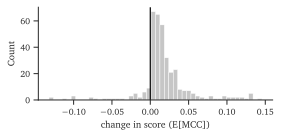
\includegraphics[keepaspectratio]{index_files/mediabag/content/part2/2-03-latent-forest-alloc_files/figure-latex/..-codefigs-results-fig-efm-mcc-output-1.pdf}}

}

\caption{\label{fig-efm-mcc}Change in Expected MCC (EFM vs FP)}

\end{figure}%

Odds of Individual Edge Improvement

\begin{figure}

\centering{

\pandocbounded{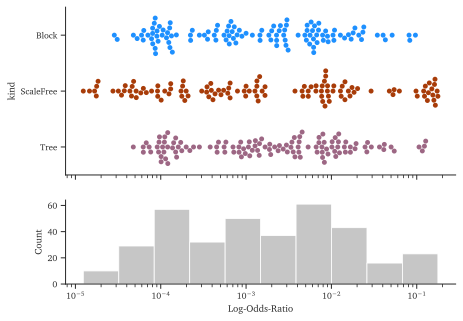
\includegraphics[keepaspectratio]{index_files/mediabag/content/part2/2-03-latent-forest-alloc_files/figure-latex/..-codefigs-results-fig-efm-logits-output-1.pdf}}

}

\caption{\label{fig-efm-logits}Logistic Regression Coef. (EFM - FP)
vs.~(Ground Truth)}

\end{figure}%

Runtime Cost

\begin{figure}

\centering{

\pandocbounded{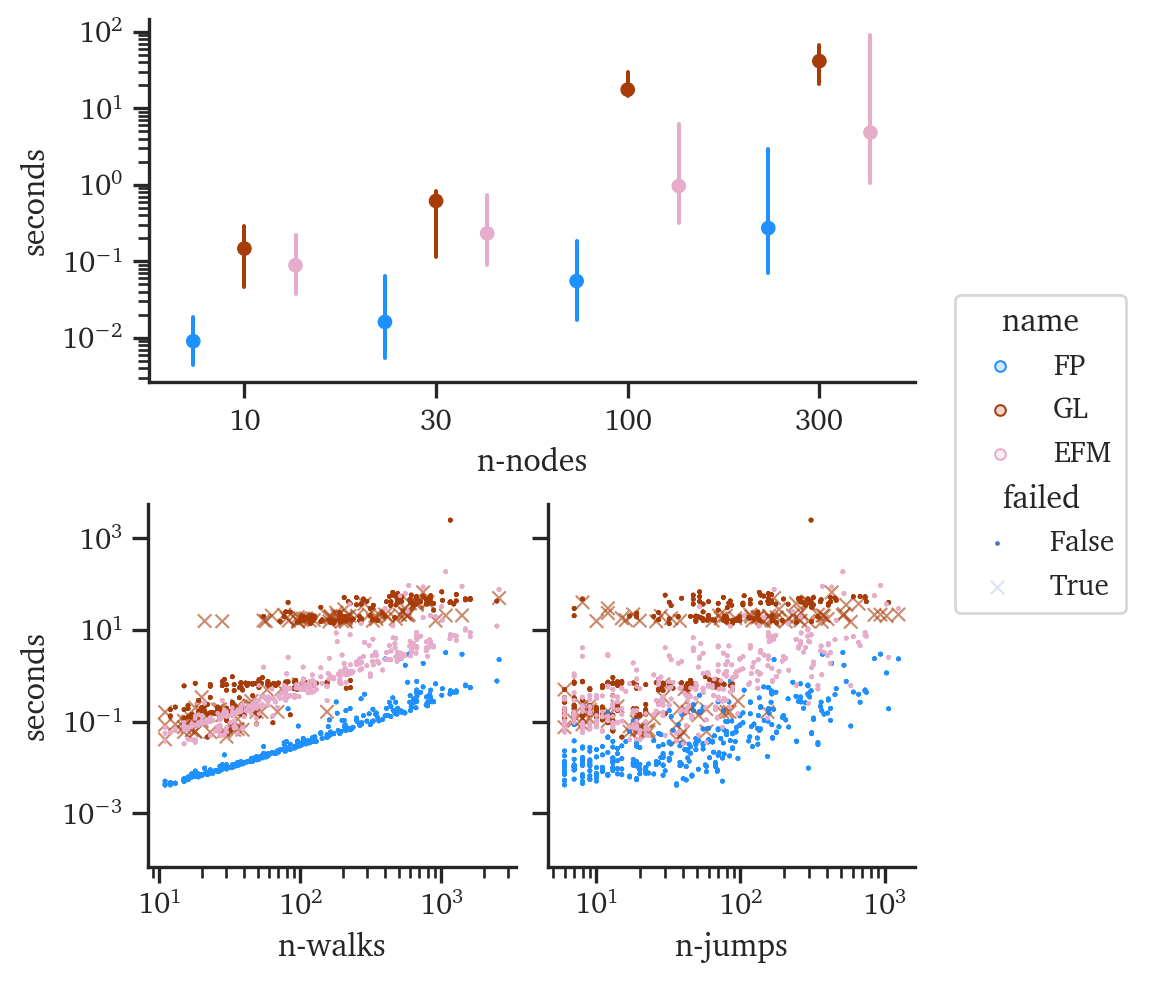
\includegraphics[keepaspectratio]{content/part2/2-03-latent-forest-alloc_files/figure-latex/..-codefigs-results-fig-efm-runtime-output-1.png}}

}

\caption{\label{fig-efm-runtime}Runtime Scaling (Forest-Pursuit vs
GLASSO)}

\end{figure}%

\begin{figure}

\centering{

\pandocbounded{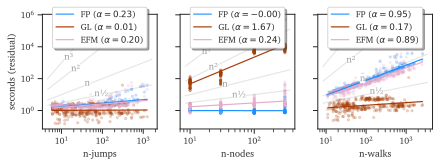
\includegraphics[keepaspectratio]{index_files/mediabag/content/part2/2-03-latent-forest-alloc_files/figure-latex/..-codefigs-results-fig-efm-partials-runtime-output-1.pdf}}

}

\caption{\label{fig-efm-partials-runtime}Partial Residuals (regression
on computation time)}

\end{figure}%

\section{Discussion}\label{discussion}

\subsection{Bayesian Estimation by Gibbs Sampling}\label{sec-lfa-gibbs}

Uniform Random Spanning Trees

\begin{itemize}
\tightlist
\item
  Methods for sampling i.e.~wilson's and Duan's (other? Energy paper?)
\item
  Tree Likelihoods, other facts (edge expectations)
\end{itemize}

Approximate Forest Samples

\begin{itemize}
\item
  comparison with LDA
\item
  Simplifying Assumptions (conditional prob IS prob for this)

  I.e. the unwritten paper, modifying technique by
  \textcite{BayesianSpanningTree_Duan2021} for RSF instead of RSTs
\end{itemize}

\part{Applications \& Extentions}

\chapter{Qualitative Application of Relationship
Recovery}\label{qualitative-application-of-relationship-recovery}

\section{Network Science Collaboration
Network}\label{network-science-collaboration-network}

\begin{figure}

\centering{

\pandocbounded{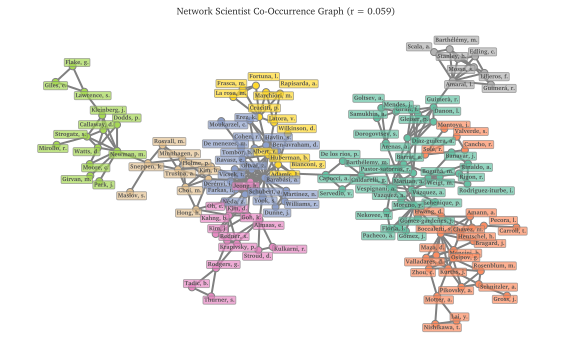
\includegraphics[keepaspectratio]{index_files/mediabag/content/part3/3-06-qualitative_files/figure-latex/..-codefigs-qualitative-fig-netsci-cooc-output-1.pdf}}

}

\caption{\label{fig-netsci-cooc}134 Network scientists from
{[}NEWMAN;BOCCALETTI;SNEPPEN{]}, connected by co-authorship}

\end{figure}%

\begin{figure}

\centering{

\pandocbounded{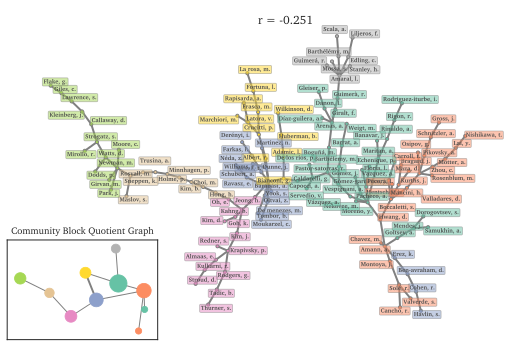
\includegraphics[keepaspectratio]{index_files/mediabag/content/part3/3-06-qualitative_files/figure-latex/..-codefigs-qualitative-fig-netsci-tree-output-1.pdf}}

}

\caption{\label{fig-netsci-tree}Max. likelihood tree dependency
structure to explain co-authorships}

\end{figure}%

\begin{figure}

\centering{

\pandocbounded{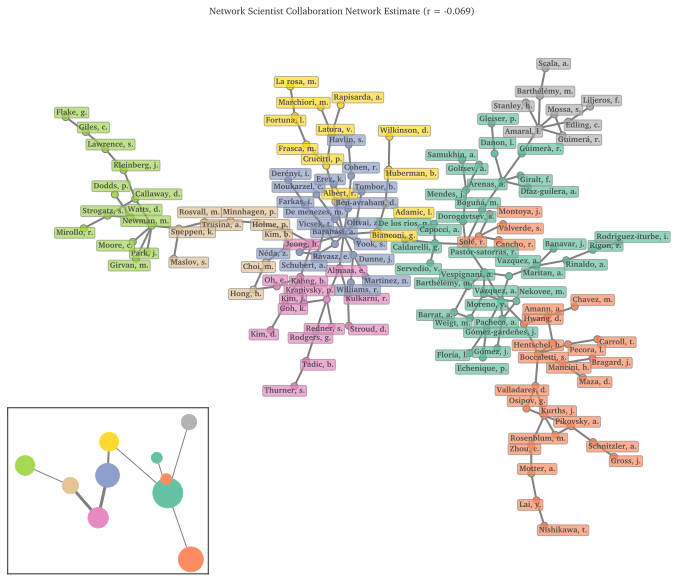
\includegraphics[keepaspectratio]{index_files/mediabag/content/part3/3-06-qualitative_files/figure-latex/..-codefigs-qualitative-fig-netsci-fp-output-1.pdf}}

}

\caption{\label{fig-netsci-fp}Forest Pursuit estimate of NetSci
collaborator dependency relationships}

\end{figure}%

\begin{figure}

\centering{

\pandocbounded{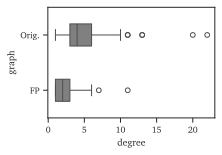
\includegraphics[keepaspectratio]{index_files/mediabag/content/part3/3-06-qualitative_files/figure-latex/..-codefigs-qualitative-fig-netsci-degree-output-1.pdf}}

}

\caption{\label{fig-netsci-degree}}

\end{figure}%

\section{Les Miserables Character
Network}\label{les-miserables-character-network}

\subsection{Backboning}\label{backboning}

\begin{figure}

\centering{

\pandocbounded{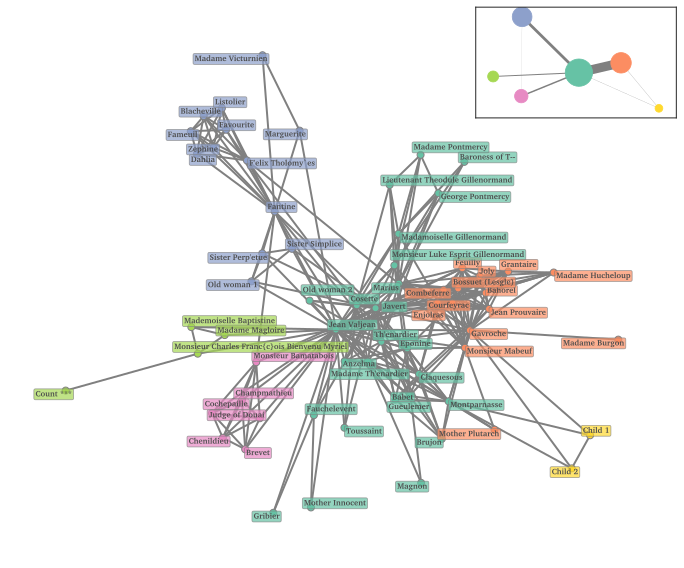
\includegraphics[keepaspectratio]{index_files/mediabag/content/part3/3-06-qualitative_files/figure-latex/..-codefigs-qualitative-fig-lesmis-cooc-output-1.pdf}}

}

\caption{\label{fig-lesmis-cooc}}

\end{figure}%

\begin{figure}

\centering{

\pandocbounded{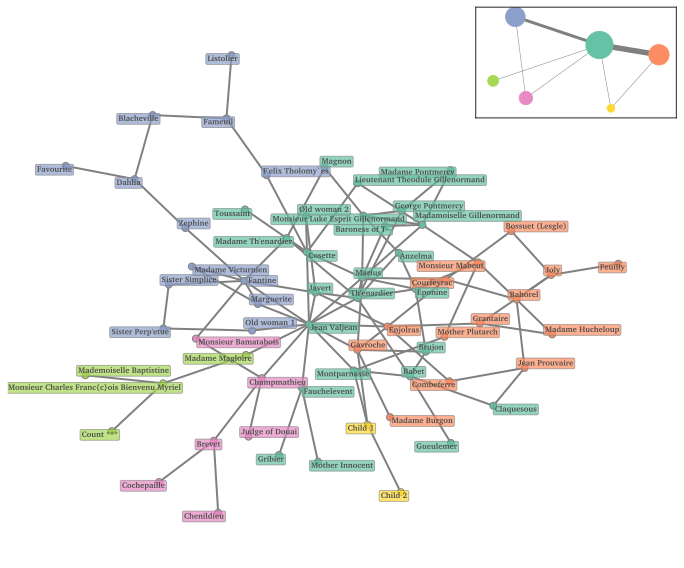
\includegraphics[keepaspectratio]{index_files/mediabag/content/part3/3-06-qualitative_files/figure-latex/..-codefigs-qualitative-fig-lesmis-fp-output-1.pdf}}

}

\caption{\label{fig-lesmis-fp}}

\end{figure}%

\subsection{Character Importance
Estimation}\label{character-importance-estimation}

\begin{figure}

\centering{

\pandocbounded{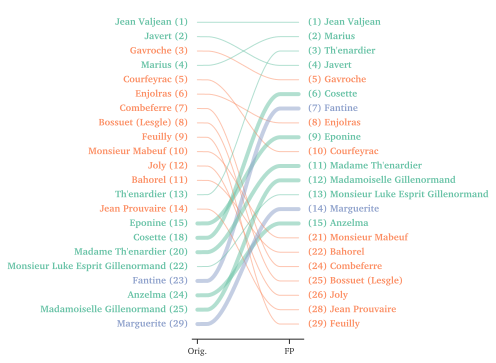
\includegraphics[keepaspectratio]{index_files/mediabag/content/part3/3-06-qualitative_files/figure-latex/..-codefigs-qualitative-fig-lesmis-centrality-output-1.pdf}}

}

\caption{\label{fig-lesmis-centrality}}

\end{figure}%

\chapter{Recovery from Partial Orders}\label{sec-ordered}

Like before, but with the added twist of \emph{knowing} our nodes were
activated with a particular partial order.

\section{Technical Language
Processing}\label{technical-language-processing}

\emph{insert from
\autocite{OrganizingTaggedKnowledge_Sexton2020,UsingSemanticFluency_Sexton2019}}

\section{Verbal Fluency Animal
Network}\label{verbal-fluency-animal-network}

\subsection{Edge Connective Effiency and
Diversity}\label{edge-connective-effiency-and-diversity}

\begin{figure}

\centering{

\pandocbounded{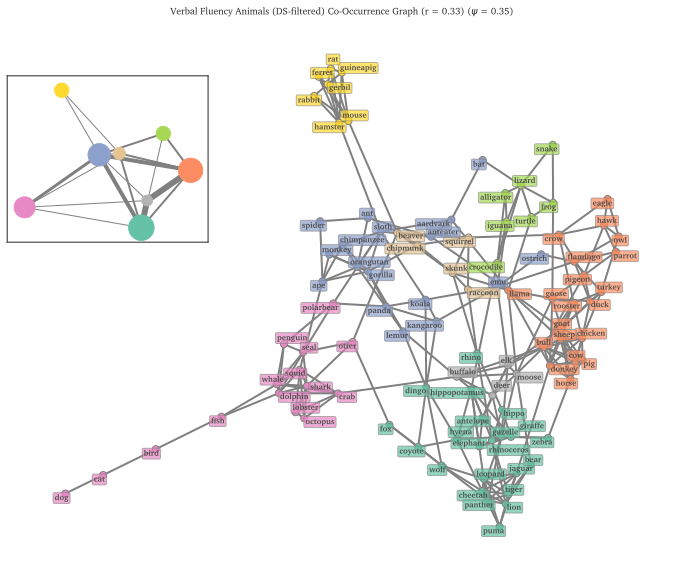
\includegraphics[keepaspectratio]{index_files/mediabag/content/part3/3-07-ordered_files/figure-latex/..-codefigs-qualitative-fig-fluency-dsmin-output-1.pdf}}

}

\caption{\label{fig-fluency-dsmin}}

\end{figure}%

\begin{figure}

\centering{

\pandocbounded{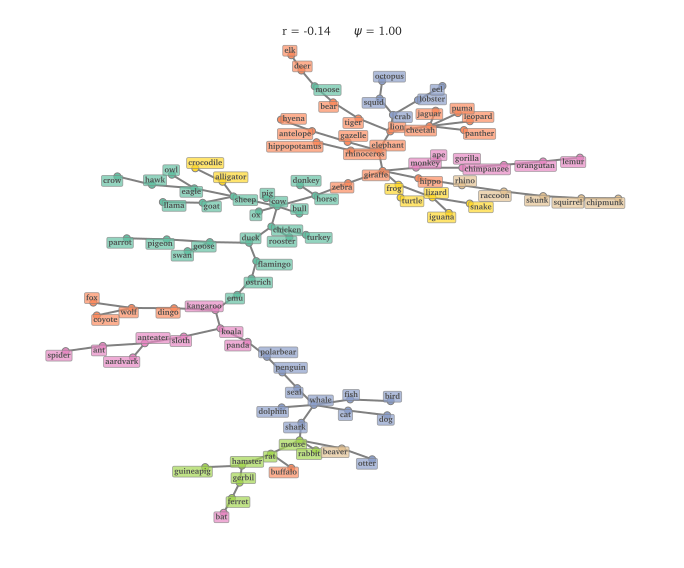
\includegraphics[keepaspectratio]{index_files/mediabag/content/part3/3-07-ordered_files/figure-latex/..-codefigs-qualitative-fig-fluency-tree-output-1.pdf}}

}

\caption{\label{fig-fluency-tree}}

\end{figure}%

\begin{figure}

\centering{

\pandocbounded{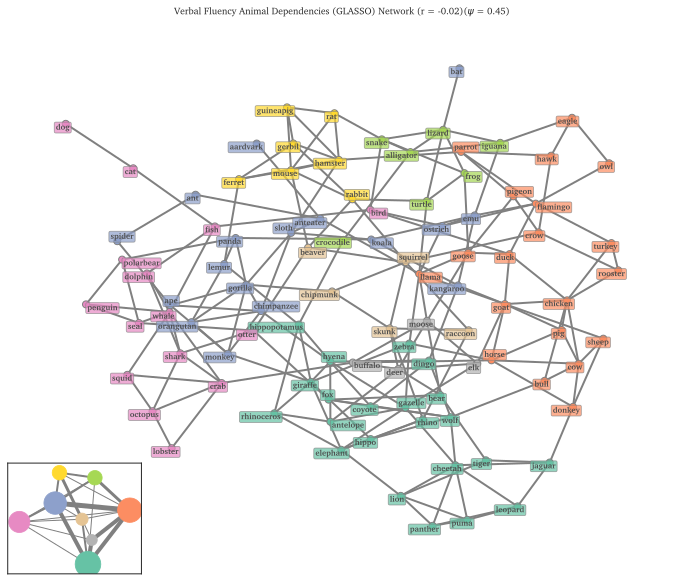
\includegraphics[keepaspectratio]{index_files/mediabag/content/part3/3-07-ordered_files/figure-latex/..-codefigs-qualitative-fig-fluency-glassomin-output-1.pdf}}

}

\caption{\label{fig-fluency-glassomin}}

\end{figure}%

\begin{figure}

\centering{

\pandocbounded{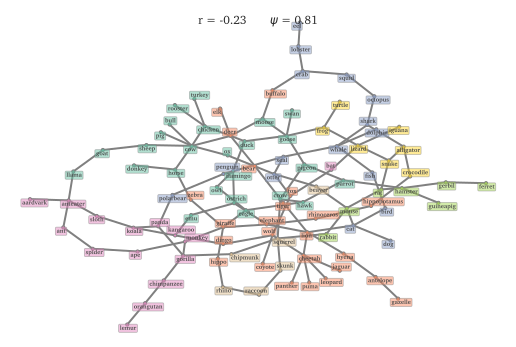
\includegraphics[keepaspectratio]{index_files/mediabag/content/part3/3-07-ordered_files/figure-latex/..-codefigs-qualitative-fig-fluency-fpmin-output-1.pdf}}

}

\caption{\label{fig-fluency-fpmin}Comparison of backboning/dependency
recovery methods tested vs.~Forest Pursuit}

\end{figure}%

\subsection{Thresholded Structure
Preservation}\label{thresholded-structure-preservation}

Differences in structural preservation with increased thresholding.

\begin{figure}

\centering{

\centering{

\pandocbounded{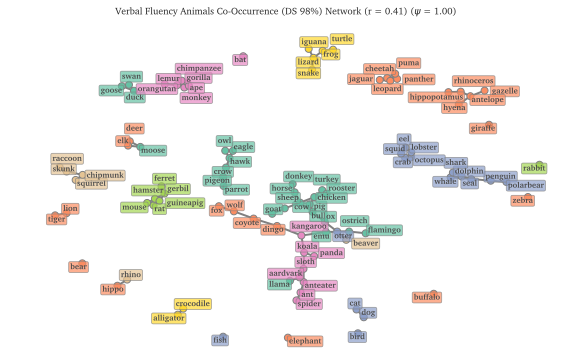
\includegraphics[keepaspectratio]{index_files/mediabag/content/part3/3-07-ordered_files/figure-latex/..-codefigs-qualitative-fig-fluency-preservation-output-1.pdf}}

}

\subcaption{\label{fig-fluency-preservation-1}co-occurrence methods will
retain local communities at the cost of global structure}

\centering{

\pandocbounded{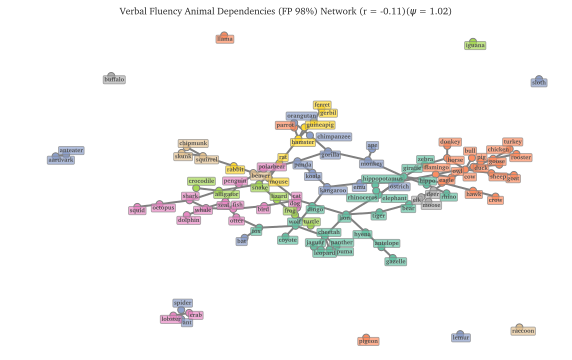
\includegraphics[keepaspectratio]{index_files/mediabag/content/part3/3-07-ordered_files/figure-latex/..-codefigs-qualitative-fig-fluency-preservation-output-2.pdf}}

}

\subcaption{\label{fig-fluency-preservation-2}dependency network drops
rarer nodes from the preserved central structure at higher uncetainty
cutoffs}

}

\caption{\label{fig-fluency-preservation}When only retaining the top 2\%
of edge strengths, blah}

\end{figure}%

\subsection{Forest Pursuit as Preprocessing}\label{sec-fp-preprocess}

Differences in structural preservation with increased thresholding.

Retaining the top 2\% of edges, co-occurrence retains local communities

at the cost of global structure.

\begin{figure}

\centering{

\centering{

\pandocbounded{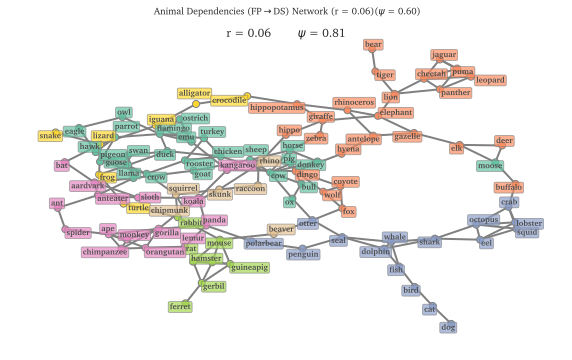
\includegraphics[keepaspectratio]{index_files/mediabag/content/part3/3-07-ordered_files/figure-latex/..-codefigs-qualitative-fig-fluency-preprocess-output-1.pdf}}

}

\subcaption{\label{fig-fluency-preprocess-1}Islands of local structure
remain (doubly-stochastic)}

\centering{

\pandocbounded{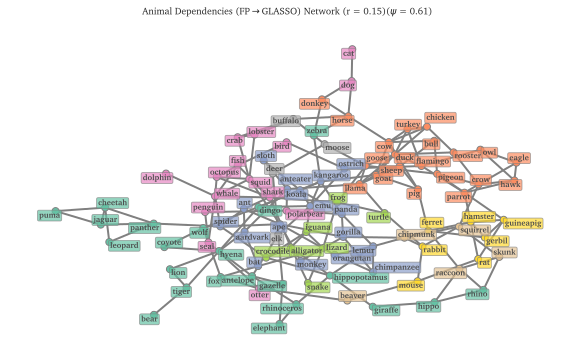
\includegraphics[keepaspectratio]{index_files/mediabag/content/part3/3-07-ordered_files/figure-latex/..-codefigs-qualitative-fig-fluency-preprocess-output-2.pdf}}

}

\subcaption{\label{fig-fluency-preprocess-2}Intact global structure with
isolates}

}

\caption{\label{fig-fluency-preprocess}We might prefer to drop
low-certainty/rare nodes from a preserved central structure.}

\end{figure}%

\chapter{Conclusion \& Future Work}\label{conclusion-future-work}

\section{Limitations of Desire Path Densities}\label{sec-issues}

\section{Modifications and Extensions to Forest
Pursuit}\label{sec-future-fp}

\section{Generalizing Inner Products on
Incidences}\label{sec-future-hyperbolic}


\singlespacing
\printbibliography

\doublespacing

\end{document}
